% !TEX root = ../thesis.tex

\chapter{Design of the Learning Environment}\label{ch:design}

In this section all implementation tools and approaches are explained.
First the used framework will be explained, then how the different scenes and objects are generated and
at last how these two are combined to the final solution: Gotscha! A learning environment based on game based learning.
The user goes through multiple levels to learn to detect and compare properties of objects
under simple and more difficult situations.

\section{Phaser 3}\label{sec:phaser-3}

Phaser\cite{phaser} is an open source HTML5\cite{html5} game framework created by Photon Storm\cite{phaser}.
It is a JavaScript/TypeScript\cite{typescript} library designed to run on all major desktop browsers.
A lot of focus was given to the performance inside of mobile web browsers.
Important for the renderer is that if the device is capable, it uses WebGL\cite{webgl}, otherwise it seamlessly reverts to Canvas\cite{canvas}.
The current version is 3.17 and is used in this work. Version 4 is in development.

\subsection{Base Configuration}\label{subsec:base-configuration}
In Phaser 3, games need a configuration file and a starting point [\ref{lst:gamesetupfile}].

\begin{lstlisting}[style=TypeScript, caption={Game Setup File}, label={lst:gamesetupfile}]
    import 'phaser';
    import GameConfig = Phaser.Types.Core.GameConfig;
    import RenderConfig = Phaser.Types.Core.RenderConfig;
    import {Scene1} from './scene1';
    import {Scene2} from './scene2';

    // Defining the renderer
    const renderConfig: RenderConfig = {
        antialias: true,
        pixelArt: false
    };

    // Enforcing widescreen
    let width: number = window.screen.width;
    let height: number = window.screen.height;

    if (window.screen.width <= window.screen.height) {
        width = window.screen.height;
        height = window.screen.width;
    }

    // Game Configuration
    const config: GameConfig = {
        title: 'TITLE',
        parent: 'game',
        type: Phaser.AUTO,
        scene: [
            scene1, scene2
        ],
        physics: {
            default: 'arcade',
            arcade: {
                debug: false
            }
        },

        // Master background color
        backgroundColor: '#000000',

        render: renderConfig,

        scale: {
            mode: Phaser.Scale.FIT,
            autoCenter: Phaser.Scale.CENTER_BOTH,
            width: width,
            height: height
        }
    };

    export class GameName extends Phaser.Game {
        constructor(config: GameConfig) {
            super(config);
        }
    }

    // Event handler for starting the game (starting point)
    window.onload = () => {
        const game = new GameName(config);
    };
\end{lstlisting}

\subsection{Scenes}\label{subsec:scenes}
Games in Phaser 3 are structured around scene objects.
A scene is a collection of game objects and related logic because these two should be kept together.
The objects will be drawn when the scene is rendered.

Where this gets special is that Phaser doesn't place any constraints on how many scenes need to be running.
This means you can have 0, 1, or as many as you need running at once.
You can communicate between them and each scene has a depth (z-index).
With the z-index a UI scene, rendered above the play scene, which is always rendered above the background scene, is possible.

\subsubsection{Lifecycle}
A simplified model has a scene that moves between four states: \textit{Create, Update Loop, Paused, and Stopped}.
Transitions are initiated by a function call and emit a signal that can be listened for.
This way, you can take action at specific point in the process.

The scene state transitions and fired events are summarized in the following state diagram.
Functions which initiate a transition are in yellow and signals emitted are orange.

\begin{figure}[H]
    \centering
    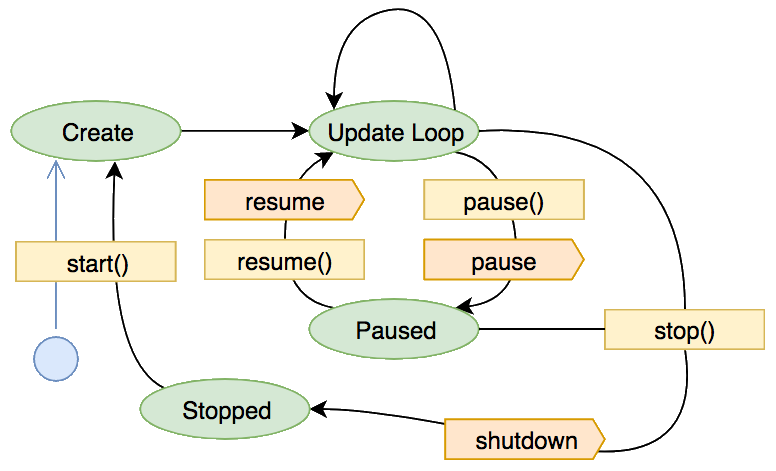
\includegraphics[width=0.8\textwidth]{figures/lifecycle}
    \caption{Scene Lifecycle\cite{phaser-guides-scenes}}
    \label{fig:lifecycle}
\end{figure}

An interesting behavior is that once a scene has been shut down it is not garbage collected.
The scene can always be resumed by the start() method.
When this happens the three creation functions get called once more.
This means any state tracked in the scene class will be retained between a stopped state and the next create state.
Thus one has to be careful with setting a known initial value on everything requiring one.
Especially when loading/creating objects outside the preloader (animations, tweens, audiofiles, etc.).

Scenes here have 5 functions:

\begin{itemize}
    \item \textbf{constructor()}: Run 1 time.
    \item \textbf{init()}: Run 1 time. Initialization of fields and passed on data by other scenes.
    \item \textbf{preload()}: Run 1 time. Loads up all the assets inside the scene like images and audio.
    \item \textbf{create()}: Run 1 time. Position and display the assets that are already preloaded, animations, physics, etc.
    \item \textbf{update()}: Run 1 time per frame, takes care of everything related to the game logic.
\end{itemize}

\subsection{Managers}\label{subsec:managers}
In Phaser 3 managers are a global system.
Animations, scenes, images loaded/created within it are globally available to all game objects.
They share the base data while managing their own timelines.
This allows the definition of a single object once and its application to as many game objects as required.
So a game object can be called in an completely other and unrelated scene.
Examples for used managers in this work are:

\begin{itemize}
    \item \textbf{Scene Manager} (scene.scenes). Contains all scenes of the game once created.
    \item \textbf{Texture Manager} (scene.textures). Contains all textures once loaded.
    \item \textbf{Audio Manager} (scene.sound). Contains all audio files once loaded.
    \item \textbf{Data Manager} (scene.data). Shared data manager.
    An event (listenable) is triggered when an event is stored/changed.
    \item \textbf{Cache Manager} (scene.cache). Contains all special files once loaded.
    \item \textbf{Animation Manager} (scene.anims). Contains all animations once created.
    \item \textbf{Tween Manager} (scene.tweens). Contains all tween objects once created.
    A Tween is able to manipulate the properties of one or more objects to any given value, based
    on a duration and type of ease.
\end{itemize}

\section{Objects}\label{sec:objects}
\subsection{Object Generation}\label{subsec:object-generation}
Our objects can have up to four properties with exactly one from each of the following categories:

\begin{itemize}
    \item \textbf{Geometrical shape} (square, triangle, circle, ellipse, rhombus, octagon)
    \item \textbf{Color} (yellow, orange, red, purple, green, blue)
    \item \textbf{Holes} or dots (one, two, three, four, five, six)
    \item \textbf{Filling} (filled, striped, dotted)
\end{itemize}

All possible objects with one, three and four properties, are needed.

With a python script [\ref{lst:svggen}] scalable vector graphic (SVG)\cite{svg-tutorial} files are generated [\ref{lst:svgimagefile}].
After that they are converted to portable network graphic (PNG) files with the GNU image manipulation program (GIMP)\cite{gimp}.
Additional image scaling and cropping is done for saving space and only displaying the actual image with as less empty space as possible around it.
With the imagemagick command \textit{mogrify} [\ref{lst:mogrify}] the last step is easily applicable to all 1000+ images.

\begin{lstlisting}[style=TypeScript, caption={SVG Generation}, label={lst:svggen}]
    ...
    imageString = imgStr(colordefault, colordark, square, circle, triangle, ellipse, octagon, rhombus, filling, one,
    two, three, four, five, six)

    filename = colordefault + shape + number + fillingname

    with open("images/svg/" + filename + ".svg", "w+") as file:
    file.write(imageString)
    file.close()
    ...
\end{lstlisting}

\begin{lstlisting}[style=TypeScript, caption={SVG Image File}, label={lst:svgimagefile}]
    <?xml version="1.0" standalone="yes"?>

    <svg height="1000" width="1000" viewbox="0 0 1000 1000" xmlns="http://www.w3.org/2000/svg">
    <defs>
    <pattern id="stripe" patternUnits="userSpaceOnUse" width="20%" height="20%">
    <path stroke="aqua" stroke-linecap="butt" stroke-width="50" d="M -20 -20 l1000 1000"/>
    ...

    </pattern>
    <pattern id="dotted" enable-background="true" patternUnits="userSpaceOnUse" width="15%" height="15%">
    <circle cx="30" cy="30" r="25" fill="aqua" />
    ...
    </pattern>
    <style>
    .button {

    stroke-width:5;
    stroke:black;

    }
    </style>
    </defs>

    <g id="circle" display="none">
    <circle cx="500" cy="500" r="300" class="button" fill="blue"/>
    ...
    </g>

    <g id="square" display="inherit">
    <rect x="250" y="250" rx="20" ry="20" width="500" height="500" class="button" fill="blue"/>
    ...
    </g>

    <g id="triangle" display="none">
    <polygon points="500,50 113.4,700 886.6,700" stroke-linejoin="round" class="button" fill="blue" />
    ...
    </g>

    <g id="ellipse" display="none">
    <ellipse cx="500" cy="500" rx="400" ry="250" class="button" fill="blue" />
    ...
    </g>
    <g id="octagon" display="none">
    <polygon points="400,250 600,250 750,400 750,600 600,750 400,750 250,600 250,400" stroke-linejoin="round" class="button" fill="blue" />
    ...
    </g>

    <g id="rhombus" display="none">
    <polygon points="350,250 150,750 650,750 850,250" stroke-linejoin="round" class="button" fill="blue" />
    ...
    </g>


    <g id="one" display="none">
    <circle cx="500" cy="500" r="40" stroke="black" fill="black"/>
    </g>

    <g id="two" display="none">
    <circle cx="570" cy="500" r="40" stroke="black" fill="black"/>
    ...
    </g>

    <g id="three" display="none">
    <circle cx="570" cy="560" r="40" stroke="black" fill="black"/>
    ...
    </g>

    <g id="four" display="none">
    <circle cx="570" cy="430" r="40" stroke="black" fill="black"/>
    ...
    </g>
    <g id="five" display="none">
    <circle cx="570" cy="430" r="40" stroke="black" fill="black"/>
    ...
    </g>

    <g id="six" display="none">
    <circle cx="570" cy="400" r="40" stroke="black" fill="black"/>
    ...
    </g>

    Sorry, your browser does not support inline SVG.
    </svg>
\end{lstlisting}

\begin{lstlisting}[style=TypeScript, caption={ImageMagick console command "mogrify"}, label={lst:mogrify}]
    mogrify -resize 50\% -trim -repage *.png
\end{lstlisting}

\subsection{Object Storage}\label{subsec:object-storage}
Our objects are images with different properties.
These properties cannot be saved in the images itself.
for that reason the image path with the respective properties are stored in a easily accessible
"JavaScript Object Notation" (JSON) [\ref{lst:json}] file.

As the game should be just a template for further graphical enhancements the JSON File can be adapted in a simple way
to other categories and images.

\textbf{IMPORTANT}: Objects in this game have three to six properties per category. This is just an example.
Categories can have more than six properties but should not have less than three.

\begin{lstlisting}[style=TypeScript, caption={JavaScript Object Notation File (geometrical\_objects.json)}, label={lst:json}]
{
  "categories": [
    {
      "name": "cat1",
      "url": "color.png",
      "validElements": [
        {
          "name": "purple",
          "urls": [
            "purple1.png",
            "purple2.png",
            ...
          ]
        },
        ...
      ]
    },
    ...
  ],
  "images": [
    {
      "name": "purplesquareonefull.png",
      "cat1": "purple",
      "cat2": "square",
      "cat3": "one",
      "cat4": "full"
    },
    ...
  ]
}
\end{lstlisting}

\subsection{Object Display}\label{subsec:object-display}
Displaying the same set of objects or just the image of an object without tweaking it a little can seem boring for the user in long term.
Thus in every game and level the set of objects is randomly selected
and playing the same game or even level keeps being visually interesting for a longer time.
To add even more diversity, objects gets a random rotation angle, size and position every time it is displayed/created.
Of course within certain predefined boundaries.
Those boundaries take into account that the minimum size should always be enough to touch it with a normal sized finger.

\subsection{Object Interaction}\label{subsec:object-interaction}
Whenever possible a generalization of the input code [\ref{lst:inputcode}] is used with every user-object interaction.
Instead of giving each object an event task, the global event task is fetched and the object via the event parameters.
This way the input interaction code is kept in one place and so less fragmented.

\begin{lstlisting}[style=TypeScript, caption={Input code}, label={lst:inputcode}]
    ...
    this.input.on('dragstart', function(pointer, gameObject) {
        ...
    }, this);

    this.input.on('drag', function(pointer, gameObject, dragX, dragY) {
        ...
    }, this);

    this.input.on('dragend', function(pointer, gameObject, dropped) {
        ...
        if (!dropped ...) {
            ...
        }
    }, this);

    this.input.on('drop', function(pointer, gameObject, dropZone) {
        ...
    }, this);
    ...
\end{lstlisting}

\subsection{Modularity}\label{subsec:modularity}
To ensure the modularity and adaptability of this work for other designs,
the objects with the property file as well as the background is completely replaceable by other images.
The subsection "Object Storage" [\ref{subsec:object-storage}] explains the most difficult part of adapting, namely
writing the property file. As a template the current property file should be used.

\section{Score Storage}\label{sec:scorestorage}
The achieved score is saved in the local storage\cite{webstorage} of the browser.
The local storage remains unchanged until it is cleared in the browser settings.
Thus the saved score is not lost on the same device until purposely deleted.
Before accessing the local storage it is checked if there even is a storage [\ref{lst:storageaccess1, lst:storageaccess2}].

\begin{lstlisting}[style=TypeScript, caption={Storage access (scoreScene.ts)}, label={lst:storageaccess1}]
    ...
    private saveScore(score: string): void {
        if (typeof(Storage) !== "undefined") {
            window.localStorage.setItem('phaser_score_' + this.previousScene, score);
        } else {
            console.log("Sorry! No Web Storage support...");
        }
    }
    ...
\end{lstlisting}

\begin{lstlisting}[style=TypeScript, caption={Storage access (levelMenuScene.ts)}, label={lst:storageaccess2}]
    ...
    if (typeof(Storage) !== "undefined") {
        if(window.localStorage.getItem('phaser_score_' + this.buttonToSceneMap(gameObject.name))){
            if (reset) {
                window.localStorage.setItem('phaser_score_' + this.buttonToSceneMap(gameObject.name), score);
            } else {
                score = window.localStorage.getItem('phaser_score_' + this.buttonToSceneMap(gameObject.name));
            }
        }
    } else {
        console.log("Sorry! No Web Storage support...");
    }
    ...
\end{lstlisting}

\section{Creating animated Introductions}\label{sec:creating-animated-introductions}
To generate animated instructions for the task later on,
the screen is recorded with the Open Broadcaster Software (OBS) Studio\cite{obs} while someone is playing the game.
Phaser does not support video playback.
Thus parts of the final video are then taken for the respective scenes and converted into single pictures.
These single pictures are saved in one picture (called spreadsheet [\ref{fig:spreadsheet}]).
Those spreadsheets can then be animated with Phaser.

Is is important to note, that different devices have a different limit for the resolution of images.
Tablets seem to have the lowest, namely 4096x4096 pixels\cite{webglmaxtexturesize}.
The spreadsheet images are scaled down for that reason.

\begin{figure}[H]
    \centering
    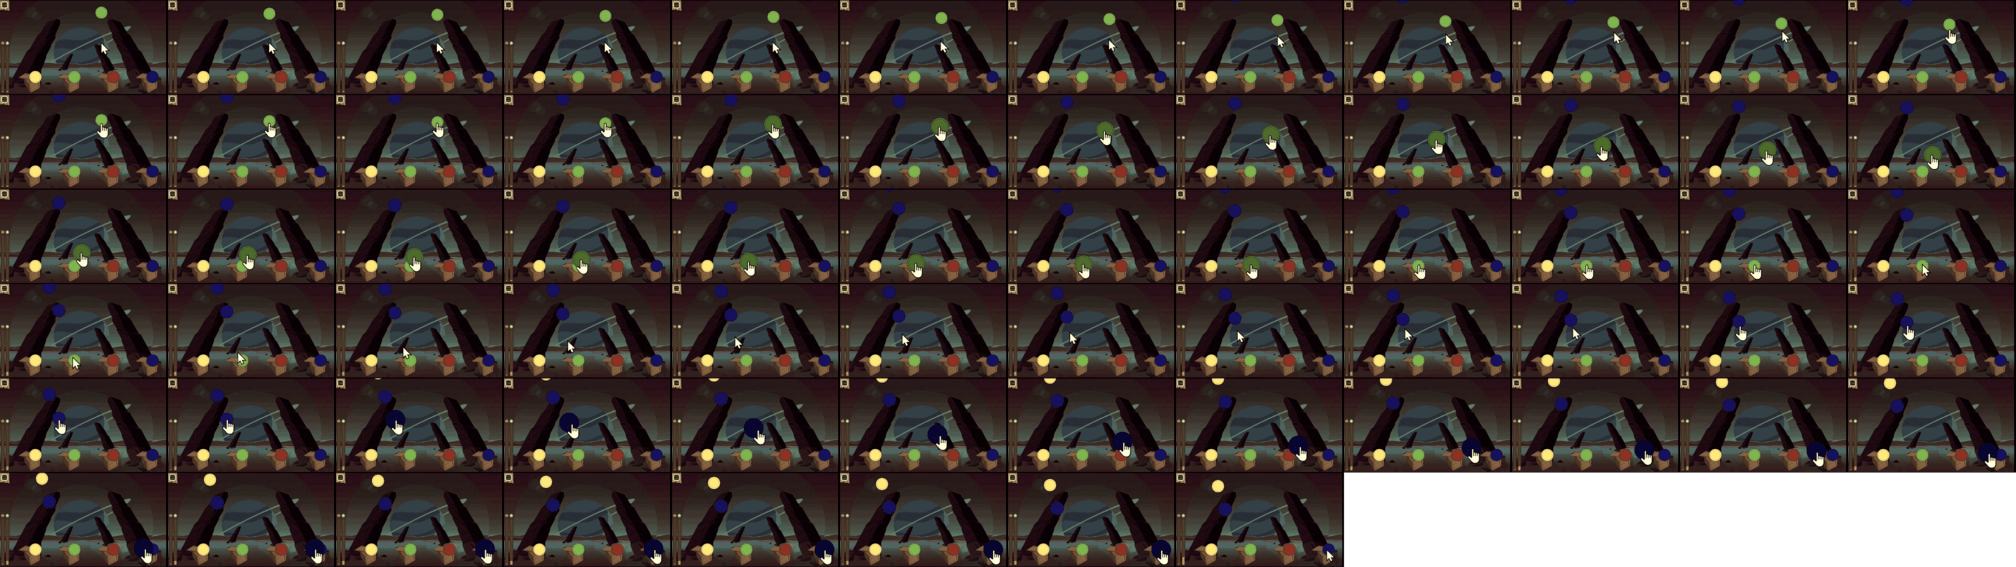
\includegraphics[width=1\textwidth]{figures/spreadsheet}
    \caption{Example: Spreadsheet}
    \label{fig:spreadsheet}
\end{figure}

\section{Scene Concept of the Learning Environment}\label{sec:scene-concept-of-the-learning-environment}
Through the given boundary conditions and requirements the environment is split into multiple parts/scenes.

\subsection{Drop Down Menu}\label{subsec:drop-down-menu}
Throughout the whole experience, the user can open a menu with a button.
This button is always visible.
Once the menu is open, the user may close the menu and return to the current scene,
exit the current scene and return to the level menu and go into fullscreen and back.
The current scene is paused while the menu is open as it can be distracting for the user,
if suddenly something pops up and covers parts of the visible and running scene.
With blurring out the current scene the user is made aware of the current scene being paused and of the "open menu" state.

\subsection{Welcome Screen}\label{subsec:welcome-screen}
The welcome screen is the starting point of the user experience.
Through this screen the user is greeted by showing the name of the game.
Through a click he may commence to the level menu.
To make the art of transition clear to the user a finger icon is displayed and animated.

\subsection{Level Menu}\label{subsec:level-menu}
In the level menu, the user is able to choose between different levels and games and can access the object summary.
Through the stars below each button the user can track his progress/score.
The progress can be resetted by the reset button.

\subsection{Object Summary}\label{subsec:object-summary}
The Object summary allows the user to get a feeling for all the different properties an object can have.
The number of objects per category is restricted to five, as there are over 1000 different objects and with all of them
the user would not be able to focus on the different properties.
Objects are draggable and sortable by each category with a click on a respective button.

\subsection{Sorting with one Category}\label{subsec:sorting-with-one-category}
Here the user has to sort the static objects with one category by the given category.
It is important for users, inexperienced with sorting objects by their properties, to start at the lowest level possible.
As the user should be able to experience all categories, they are split into different levels.
Each level represents a category.

For motivational purposes, the user can track his progress.
The Progress is defined by objects sorted the right and the wrong way.

The amount of objects to sort, as well as the amount of properties of the category
is randomly selected each time you start the game.

\subsection{Sorting with one Category under difficult Conditions}\label{subsec:sorting-with-one-category-under-difficult-conditions}
It is important to internalize learned skills under difficult conditions.
This turns mental processes into automatisms, which means to execute processes correctly without thinking.

So in this game the user has to sort falling objects with one category by the given category.
As the user should be able to experience all categories, they are split into different levels.
Each level represents a category.

For motivational purposes, the user can track his progress.
The progress is defined by objects missed, sorted the right and the wrong way.
To make the task harder, objects get instead of a randomly selected rotation angle a randomly selected spin velocity.
Dummy objects are added as well.
Those objects look similar to the original ones but with a succinct characteristic.
There are no negative points for missing such an object but negative points for sorting them in any way.

For more diversity, the amount of falling objects to sort, as well as the amount of properties of the category
is randomly selected each time you start the game.

\subsection{Sorting with restricted space}\label{subsec:sorting-with-restricted-space}
This game scene is specific designed for the users preparation to the computer science topic hashing or hash functions.

A hash function is any function that can be used to map data of arbitrary size to fixed-size values.
The values returned by a hash function are called hash values, hash codes, or simply hashes and
are used to index a fixed-size table called a hash table.
The use of a hash function to index a hash table is called hashing or scatter storage addressing.\cite{artofcomputerscience}

Broadly summarized, a hash function converts a given sequence of objects (e.g.\ text, symbols, etc.)
with a certain length to a fixed sequence with always the same length within the same hash function.
This function is not invertible.

This scene is an strong abstraction of a hash function.
The user has to sort a given number of objects, with all properties shown, into boxes with limited space.

The objects in one box must have at least one property in common and
can be put into the box and taken out an infinite amount of times.

To make the game more difficult, this level is split into two.
The first level has boxes with the size 6, 4, 2 and the second one boxes with the size 6, 5, 4.

\subsection{Object pairing}\label{subsec:object-pairing}
This game scene trains the user in the comparison and grouping of objects.
In the process he must identify and isolate properties of different objects, compare them and remember the outcome.
To finally compare objects and reach a conclusion if the objects can be grouped or not,
the user has to remember multiple outcomes.

This lays a foundation of a rich mathematical structure linking it to the combinatorics of finite affine and
projective spaces and the theory of error-correcting codes.\cite{cardgameset}

The game is split into two versions. The easy one for adapting to the correct thinking
and the normal one to strengthen it.

There are twelve objects being displayed.
The user has to select three objects which have to fulfill the following rules.

For each category one of the following conditions has to hold:
\begin{itemize}
    \item They must be the same (blue, blue, blue)
    \item They must be completely different (square, triangle, circle)
\end{itemize}

If the user needs help, there is a helper bar which can be accessed by a button with a question mark on it.
The helper bar shows which categories fulfill the conditions and which do not
by coloring the category symbols on the bar in green or red.

The game is time limited. The remaining time is shown by a bar.
If you select three objects which fulfill the conditions, more time will be added.
After a set amount of correct selected objects, the game will end.

If there are no three objects that fulfill the conditions, the play field will be generated anew.

\subsubsection{Object pairing - easy version}\label{subsubsec:object-pairing---easy-version}
In the easy version objects have three categories: \textit{color, shape and number of holes/dots}

\begin{figure}[H]
    \centering
    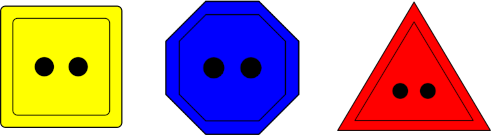
\includegraphics[width=0.5\textwidth]{figures/matchingseteasy}
    \caption{Example: Matching Set Easy}
    \label{fig:matchingseteasy}
\end{figure}

\subsubsection{Object pairing - hard version}\label{subsubsec:object-pairing---hard-version}
In the hard version objects have four categories: \textit{color, shape, number of holes/dots and filling}

\begin{figure}[H]
    \centering
    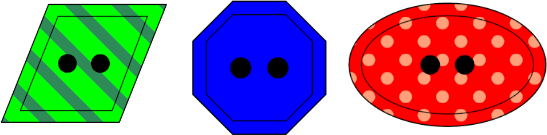
\includegraphics[width=0.5\textwidth]{figures/matchingsethard}
    \caption{Example: Matching Set Hard}
    \label{fig:matchingsethard}
\end{figure}

\subsection{Score Screen}\label{subsec:score-screen}
After the completion of a task/level/game, the user will be granted a score.
The score is represented here with a displayed number of stars.
The minimum of stars is zero and the maximum is three.
If the user is unhappy with his results, he can replay the game by clicking on the replay button.
To return back to the level menu the user has to click anywhere on the screen (excluding buttons).
To make this action clear, a clicking finger is being displayed.

\subsection{Introduction}\label{subsec:introduction}
As the task beforehand for each level may not be clear to every user an introduction is necessary.
Before each game starts, an animation [\ref{sec:creating-animated-introductions}] of the task beforehand is being shown.
This scene serves as a helper scene so that the running scene can be paused while the animated introduction runs.
If the current scene is not paused in the meantime, the user may not take enough time to understand the task.

\section{Code structure of the learning environment}\label{sec:code-structure-of-the-learning-environment}
Our learning environment consists of different scenes each one inherits the base scene.
The following subsections contain a summary of crucial and not trivial parts of the code.

The full code can be accessed in the appendix [\ref{ch:gotcha!---full-codegot}] or on gitlab\cite{gitlab-thesis}.

\begin{figure}[H]
    \centering
    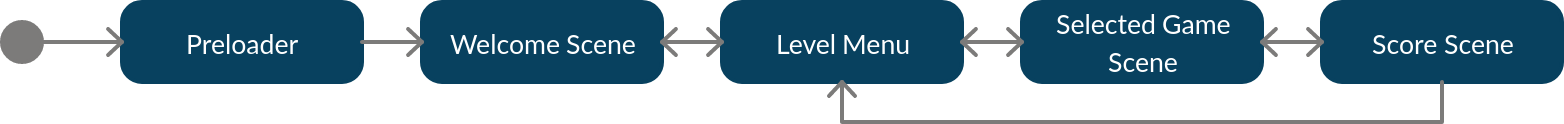
\includegraphics[width=1\textwidth]{figures/statediagram}
    \caption{Scene State Diagram}
    \label{fig:statediagram}
\end{figure}

\subsection{Playing the Game}\label{subsec:playing-the-game}
The game can be played here\cite{gotscha}.

\subsection{Running the Code}\label{subsec:running-the-code}
To run the code clone the gitlab repository\cite{gitlab-thesis} and run the following commands in the terminal in the cloned folder.

\begin{lstlisting}[style=TypeScript, caption={BaseScene.ts}]
    npm run start
\end{lstlisting}

The game should now be playable on \textbf{"localhost:8080"} in a web browser of your choosing.

Please note that the gameplay video is not included in the repository.

\subsection{BaseScene}\label{subsec:basescene}
This scene contains methods and fields which are necessary in multiple scenes
(e.g.\ the scene transition, identifier of the scene, ...).

\subsubsection{The Scene Transition}
Transitions are simply made by laying a geometrical mask over an game object and animate the mask.
As masks have to be applied to every object they have to mask,
a simple solution was to lay a black rectangle over the whole scene and mask it.
So the scene transition has the form of a circle cut out of a black rectangle [\ref{lst:transitioninitializationmethod}].
The animation comes to life with increasing or decreasing
the radius of the circle according to the wanted animation (IN/OUT).

\begin{lstlisting}[style=TypeScript, caption={Transition Initialization Method (BaseScene.ts)}, label={lst:transitioninitializationmethod}]
    ...
    private transitionInit(): void {
        // Shape of the graphical transition
        const circle: Phaser.GameObjects.Graphics = this.add.graphics();

        // Shape of the screen
        const rectangle: Phaser.GameObjects.Rectangle = this.add.rectangle(0, 0, this.cameras.main.width, this.cameras.main.height, 0x000000);

        // Define circle as the mask
        const mask: Phaser.Display.Masks.GeometryMask = circle.createGeometryMask();

        circle.setPosition(this.cameras.main.width / 2, this.cameras.main.height / 2);
        circle.fillCircle(0, 0, 0.1);
        circle.setDepth(0);

        mask.setInvertAlpha(true);

        rectangle.setDepth(1);
        rectangle.setOrigin(0, 0);
        rectangle.setMask(mask);

        circle.fillCircle(0, 0, 0.1);

        this.transition = [circle, rectangle];
    }
    ...
\end{lstlisting}

\subsection{PreloadAssets}\label{subsec:preloadassets}
In the "preload()" method the files used later on can be loaded into the respective managers/cache.
Now every asset loaded this way has a unique identifier and can be used in future scene
as long as it is not removed explicitly.
The asset can as such be loaded into the managers/cache in every scene,
so that only the actual used assets are loaded.
The advantage of this is that you can save time and storage.
But the disadvantage is that you have to be connected to the internet the whole time.
Should the connection be severed for only a short time, objects might not be displayed correctly.
With a "preloadAsset" scene in the beginning, all available assets are loaded,
so that after the longer loading time the game can run fluently,
without problems and most importantly without a connection to the internet.

The attributes and path of objects in the imported json file [\ref{subsec:object-generation}]
can be accessed by filename.["fieldname"] or filename.fieldname [\ref{lst:jsonfileaccess}].

\begin{lstlisting}[style=TypeScript, caption={Example json file access}, label={lst:jsonfileaccess}]
    ...
    for (let category of loadedJsonObjectFile['categories']) {
        console.log("URL: " + category['url']);
        console.log("Name: " + category['validElements']['name']);
        console.log("ValidElement urls: " + category['validElements']['urls']);
    }

    for (let image of loadedJsonObjectFile['images']) {
        console.log("Name: " + image.name);
        console.log("Cat1: " + image.cat1);
        ...
    }
    ...
\end{lstlisting}

The way the objects files are preloaded into the respective managers is shown below [\ref{lst:jsonpreload}].
It is important to note that if assets are loaded outside of the preload() method,
the loader has to be started manually.

\begin{lstlisting}[style=TypeScript, caption={preloadAsset.ts}, label={lst:jsonpreload}]
    ...
    private preload(): void {
        this.load.setPath('assets/geometrical_objects/');
        this.load.json('objects', 'geometrical_objects.json');
        ...
    }
    ...
    private create(): void {
        ...
        this.preLoadImages();
        ...
        this.start();
    }
    ...
    private preLoadImages(): void {
        // Load category and object images
        const jsonObject: any = this.cache.json.get('objects');

        for (let category of jsonObject['categories']) {
            this.load.setPath('assets/geometrical_objects/categories/');
            this.load.image(category['name'], category['url']);

            this.load.setPath('assets/geometrical_objects/images/');
            for (let property of category['validElements']) {
                for (let url of property['urls']) {
                    this.load.image(url, url);
                }
            }
        }

        for (let image of jsonObject['images']) {
            this.load.image(image['name'], image['name']);
        }
        ...
    }
    ...
    private start(): void {
        ...
        this.load.start();
    }
    ...
\end{lstlisting}

\subsubsection{Image Game Objects}
Instead of representing an image as a normal image in game, sprites, a special texture, is used.
But what is a sprite?
A sprite is a game object which can display both static and animated images in your game.
The big main difference between a sprite and an image game object is that you cannot animate images.
Additionally, sprites have input events, additional functions, fields and physics bodies.

\subsection{DropDownMenu}\label{subsec:dropdownmenu}
In this scene the drop down menu is created.
The scene is never stopped and is always on top of other scenes.

The following code [\ref{lst:sceneback}] in every other scene ensures this:
\begin{lstlisting}[style=TypeScript, caption={Send current scene to back}, label={lst:sceneback}]
    ...
    create(): void {
        this.game.scene.sendToBack(this.getKey());
        ...
    }
    ...
\end{lstlisting}

As the drop down animation takes time, it was necessary to create a boolean field as a lock.
This ensures that the closing and opening animation won't interfere with each other.
The lock is freed after the completion of an event/animation.

\begin{lstlisting}[style=TypeScript, caption={Lock acquiring and freeing}]
    ...
    if (!this.lock) {
        this.lock = true;
        ...
    }
    ...
    onComplete: () => this.lock = false;
    ...
\end{lstlisting}

While the menu is down/open, the current scene has to be paused.
This is achieved by accessing the other scene by fetching the key of the only other active scene and pausing it.
Important to note is, that the last started/activated scene is at position 0 in the array of all active scenes.
\begin{lstlisting}[style=TypeScript, caption={Fetching current active scene}]
    ...
    const key_paused_scene: string = this.game.scene.getScenes(true)[0].key;
    this.game.scene.pause(key_paused_scene);
    this.key_paused_scene = key_paused_scene;
    ...
\end{lstlisting}

The same trick is used for closing all current scenes when exiting (without the dropDownMenu Scene).

\subsection{LevelMenuSceneScene}\label{subsec:levelmenuscenescene}
Levels with the same difficulty are distinguished by numbers from one to four.
Those with another difficulty are distinguished by images of monsters with different level of spookiness
[\ref{fig:easylevelicon, fig:mediumlevelicon, fig:hardlevelicon}].

\begin{figure}[H]
    \centering
    
\includegraphics[width=0.2\textwidth]{figures/easylevelicon}
    \caption{Easy Level Icon}
    \label{fig:easylevelicon}
\end{figure}

\begin{figure}[H]
    \centering
    
\includegraphics[width=0.2\textwidth]{figures/mediumlevelicon}
    \caption{Medium Level Icon}
    \label{fig:mediumlevelicon}
\end{figure}

\begin{figure}[H]
    \centering
    
\includegraphics[width=0.2\textwidth]{figures/hardlevelicon}
    \caption{Hard Level Icon}
    \label{fig:hardlevelicon}
\end{figure}

As there are multiple buttons in this scene it is important to simulate a specific button behaviour.
A click is split into "pointer up" and "pointer down" and thus can vary in its combinations on where those events happen.

\begin{enumerate}
    \item pointer down and pointer up in the same button area
    \item pointer down and pointer up in different button areas
    \item pointer down and pointer up where only pointer down is in a button area
    \item pointer down and pointer up where only pointer up is in a button area
\end{enumerate}

To make sure that the behaviour is bug free, on pointer down on a button, this respective button is marked [\ref{lst:buttonmarking}].
Now, only marked buttons can react to pointer up events.
And upon any pointer up event all markers are removed.

\begin{lstlisting}[style=TypeScript, caption={Button marking (levelMenuScene.ts), label={lst:buttonmarking}}]
    ...
    private initInput(): void {
        this.input.on('pointerdown', function(pointer, currentlyOver) {
            const gameObject: any = currentlyOver[0];
            if (gameObject instanceof Phaser.GameObjects.Sprite) {
                ...
                gameObject.setData('clicked', true);
            }
        }, this);

        this.input.on('pointerup', function(pointer, currentlyOver) {
            const gameObject: any = currentlyOver[0];
            if (gameObject instanceof Phaser.GameObjects.Sprite && gameObject.getData('clicked')) {
                this.buttonFunction(gameObject);
            }

            this.levelButtons.getChildren().forEach(function(gameObject) {
                if (gameObject instanceof Phaser.GameObjects.Sprite) {
                    ...
                    gameObject.setData('clicked', false);
                }
            }, this);
        }, this);
    }
    ...
\end{lstlisting}

\subsection{IntroScene}\label{subsec:introscene}
To pause the current scene and still play the animated introduction, a separate scene is necessary.
Each time an intro has to be played, the intro scene is started anew.
The current scene is pauses itself when the intro scene is started and the name/key/identifier
of the paused scene is given to the intro scene.
That way the intro scene can resume the paused scene and then stop itself.

The respective intro material is selected via the name/key/identifier of the paused scene.

\subsection{SortingScene}\label{subsec:sortingscene}
To sort the displayed objects by their respective subcategory by clicking on one of the category buttons,
random coordinates [\ref{lst:returnquad}] are needed dependant on the screen size and object size.

\begin{lstlisting}[style=TypeScript, caption={returnQuad() (sortingScene.ts)}, label={lst:returnquad}]
    ...
    private returnQuad(quadrant: number, quadrantType: number): number[] {
        let ret: number[] = null;
        ...
        const leftOffsite: number = 100;
        const rightOffsite: number = 0;
        const topOffsite: number = 0;
        const bottomOffsite: number = 100;

        // Has entries dependant of
        const horizontal: number[] = [];

        // Has numberOfLines + 1 entries
        const vertical: number[] = [];

        horizontal.push(leftOffsite);

        vertical.push(topOffsite);

        switch (quadrantType) {
            case 3: {
                horizontal.push(leftOffsite + (this.cameras.main.width - leftOffsite - rightOffsite) / 3);
                horizontal.push(leftOffsite + (this.cameras.main.width - leftOffsite - rightOffsite) * 2 / 3);
                break;
            }
            case 4: {
                horizontal.push(leftOffsite + (this.cameras.main.width - leftOffsite - rightOffsite) / 2);
                vertical.push(topOffsite + (this.cameras.main.height - topOffsite - bottomOffsite) / 2);
                break;
            }
            case 6: {
                horizontal.push(leftOffsite + (this.cameras.main.width - leftOffsite - rightOffsite) / 3);
                horizontal.push(leftOffsite + (this.cameras.main.width - leftOffsite - rightOffsite) * 2 / 3);
                vertical.push(topOffsite + (this.cameras.main.height - topOffsite - bottomOffsite) / 2);
                break;
            }
            default: {
                break;
            }
        }

        horizontal.push(this.cameras.main.width - rightOffsite);
        vertical.push(this.cameras.main.height - bottomOffsite);

        switch (quadrantType) {
            case 3: {
                ret = [Phaser.Math.RND.between(horizontal[quadrant] + spriteSizeHalf, horizontal[quadrant + 1] - spriteSizeHalf), Phaser.Math.RND.between(vertical[0] + spriteSizeHalf + this.cameras.main.height / 8, vertical[1] - spriteSizeHalf - this.cameras.main.height / 8)];
                break;
            }
            case 4: {
                if (quadrant < 2) {
                    ret = [Phaser.Math.RND.between(horizontal[quadrant] + spriteSizeHalf, horizontal[quadrant + 1] - spriteSizeHalf), Phaser.Math.RND.between(vertical[0] + spriteSizeHalf, vertical[1] - spriteSizeHalf)];
                } else {
                    ret = [Phaser.Math.RND.between(horizontal[quadrant \% 2] + spriteSizeHalf, horizontal[(quadrant \% 2) + 1] - spriteSizeHalf), Phaser.Math.RND.between(vertical[1] + spriteSizeHalf, vertical[2] - spriteSizeHalf)];

                }
                break;
            }
            case 6: {
                if (quadrant < 3) {
                    ret = [Phaser.Math.RND.between(horizontal[quadrant] + spriteSizeHalf, horizontal[quadrant + 1] - spriteSizeHalf), Phaser.Math.RND.between(vertical[0] + spriteSizeHalf, vertical[1] - spriteSizeHalf)];
                } else {
                    ret = [Phaser.Math.RND.between(horizontal[quadrant \% 3] + spriteSizeHalf, horizontal[(quadrant \% 3) + 1] - spriteSizeHalf), Phaser.Math.RND.between(vertical[1] + spriteSizeHalf, vertical[2] - spriteSizeHalf)];
                }
                break;
            }
            default: {
                break;
            }
        }
        return ret;
    }
\end{lstlisting}

\subsection{PropertySortingScene}\label{subsec:propertysortingscene}
To specify the difficulty level, two fields are needed:
\begin{lstlisting}[style=TypeScript, caption={Level fields (propertySortingScene.ts)}]
    ...
    private setCat: number;
    ...
    private infinite: boolean;
    ...
\end{lstlisting}

In contrast to other scenes, objects must have the type Phaser.Physics.Arcade.Sprite as only arcade sprites have the
possibility of an acceleration in a direction.

As additional visual feature objects get a random spin velocity and the time an object spawns gets shorter over time.

\subsection{RestrictedSortingScene}\label{subsec:restrictedsortingscene}
To check if objects in the same box have some property in common,
the four properties of an object are taken as a list of strings and intersected with the list of strings from the other
objects in the same box [\ref{lst:equalitycheckres}].
If finally there is no empty list, the objects have some property in common and thus this is a valid solution for one box.
Which one does not matter to us in this case.
That way, the possibility of multiple solutions, which were not intended but also correct, is open.

\begin{lstlisting}[style=TypeScript, caption={equalityCheck (restrictedSortingScene.ts)}, label={lst:equalitycheckres}]
    ...
        private equalityCheck(gameObject: Phaser.GameObjects.Sprite, dropZone: Phaser.GameObjects.Zone): boolean {
        ...
        let mergeArray: any[] = [];
        ...
        for (let cat of this.jsonObject['categories']) {
            mergeArray = [...mergeArray, ...cat['validElements']];
        }
        mergeArray.forEach((element, index, array) => array[index] = element.name);
        ...
        [...this.objZoneMap.filter((element, index) => this.zoneObjMap[index].name === dropZone.name), gameObject].forEach(function (element) {
            mergeArray = mergeArray.filter((x) => element.getData('properties').includes(x));
        });
        ...
        return (mergeArray.length > 0);
    }
    ...
\end{lstlisting}

\subsection{GameScene}\label{subsec:gamescene}
In the game scene, three marked objects are checked for equality
if the respective method was not already run for exactly those three objects [\ref{lst:update}].

\begin{lstlisting}[style=TypeScript, caption={update (gameScene.ts)}, label={lst:update}]
    ...
    update(time: number): void {
        ...
        if (!this.checked && this.arrayMarked.getLength() >= 3) {
            this.checked = true;
            ...
        }
        ...
        if (timedata <= 0) {
            this.checked = true;

            ...
        } else {
            timedata -= this.timedataStepsize;
            this.timefluid.setData('timeY', timedata);
            this.timefluid.setScale(this.timefluid.getData('timeX'), timedata);
        }
    }
\end{lstlisting}

The maximum score 'gameMax' is calculated with a quotient.
Therefore there is a rounding error in the floating point arithmetic.
To even this error epsilon, the maximum relative error of the rounding procedure, has to be added or subtracted.

\begin{lstlisting}[style=TypeScript, caption={updateProgressbar (gameScene.ts)}]
    ...
    if (this.points >= this.gamefluid.getData('gameMax') - Phaser.Math.EPSILON) {
        ...
    }
    ...
\end{lstlisting}

The helpers menu icons have to be marked according to the selected three objects.
Therefore the checkEquality method [\ref{lst:checkequalitygame}] is modified with a boolean to mark the icons while executing the check.

\begin{lstlisting}[style=TypeScript, caption={checkEquality (gameScene.ts)}, label={lst:checkequalitygame}]
    ...
    private checkEquality(sprite1: Phaser.GameObjects.GameObject, sprite2: Phaser.GameObjects.GameObject, sprite3: Phaser.GameObjects.GameObject, inGame: boolean): boolean {
        if (sprite1 instanceof Phaser.GameObjects.Sprite &&
            sprite2 instanceof Phaser.GameObjects.Sprite &&
            sprite3 instanceof Phaser.GameObjects.Sprite
        ) {
            // Return value
            let replaceObjects: boolean = true;

            for (let categoryIndicator of this.arrayCategory.getChildren()) {

                // Make sure your objects are sprites
                if (categoryIndicator instanceof Phaser.GameObjects.Sprite) {

                    // Clear tint
                    categoryIndicator.clearTint();

                    if (
                        sprite1.getData(categoryIndicator.name) === sprite2.getData(categoryIndicator.name) &&
                        sprite2.getData(categoryIndicator.name) === sprite3.getData(categoryIndicator.name) &&
                        sprite1.getData(categoryIndicator.name) === sprite3.getData(categoryIndicator.name)
                    ) {
                        if (inGame) {
                            categoryIndicator.setTintFill(0x00dd00);
                        }
                    } else if (
                        !(sprite1.getData(categoryIndicator.name) === sprite2.getData(categoryIndicator.name)) &&
                        !(sprite2.getData(categoryIndicator.name) === sprite3.getData(categoryIndicator.name)) &&
                        !(sprite1.getData(categoryIndicator.name) === sprite3.getData(categoryIndicator.name))
                    ) {
                        if (inGame) {
                            categoryIndicator.setTintFill(0x00dd00);
                        }
                    } else {
                        if (replaceObjects) {
                            replaceObjects = false;
                        }
                        if (inGame) {
                            // Mark category as red
                            categoryIndicator.setTintFill(0xdd0000);
                        }
                    }
                }
            }
            return replaceObjects;
        }
    }
\end{lstlisting}

To add another small gamification element in the form of a mini reward to the game, every time the user finds a matching
pair, some additional is added to the timer [\ref{lst:updateprogress}]. So the user is even more motivated to find pairs even faster.
But not only that, the user sets himself under stress and thus the game gets harder without making it actually harder.

\begin{lstlisting}[style=TypeScript, caption={updateProgressbar (gameScene.ts)}, label={lst:updateprogress}]
    ...
    let timedata: number = this.timefluid.getData('timeY');
    timedata += this.timedataStepsize * 5000;
    if (timedata > this.timefluid.getData('timeYMax')) {
        timedata = this.timefluid.getData('timeYMax');
    }
    ...
\end{lstlisting}

It is frustrating to not find a matching pair, thus
it is ensured [\ref{lst:refresh}] that there is at least one possible pair every time a new object is added.

\begin{lstlisting}[style=TypeScript, caption={Refreshing the current set of objects (gameScene.ts)}, label={lst:refresh}]
    ...
    private rebuildDisplayedObjects(): void {
        ...
        for (let card of this.arrayDisplayed.getChildren()) {
            if (card instanceof Phaser.GameObjects.Sprite) {
                card.setVisible(false);
                this.arrayStack.add(card);
            }
        }

        this.arrayDisplayed.clear(false, false);

        this.initObjects();
    }
    ...
\end{lstlisting}

\subsection{ScoreScene}\label{subsec:scorescene}
The most important and special part in the score scene is the way the score is saved,
as explained in the score storage section [\ref{sec:scorestorage}].

\section{Final Look of the Learning Environment}\label{sec:final-look-of-the-learning-environment}
This section contains the final look of the learning environment.

\begin{figure}[H]
    \centering
    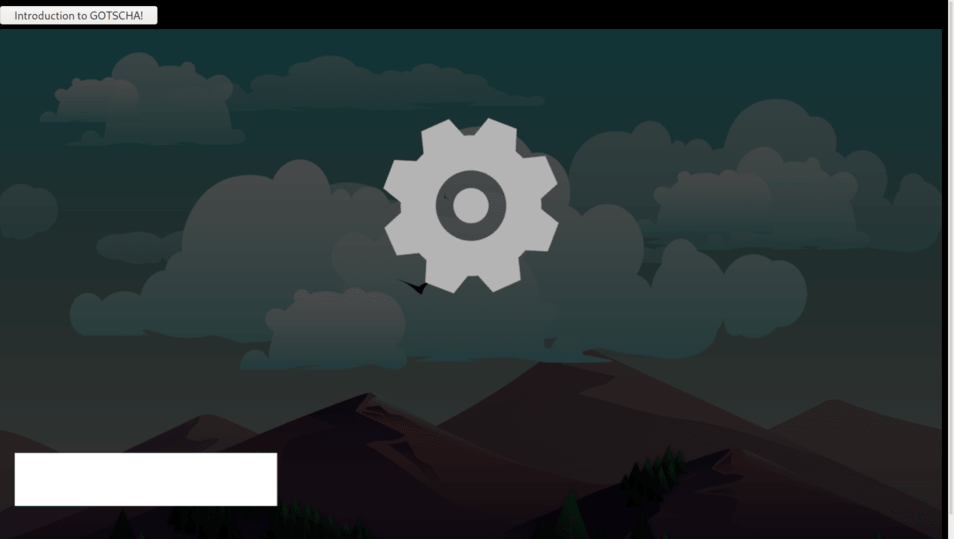
\includegraphics[width=1\textwidth]{figures/loadingscreen}
    \caption{Loading Screen}
    \label{fig:loadingscreen}
\end{figure}

\begin{figure}[H]
    \centering
    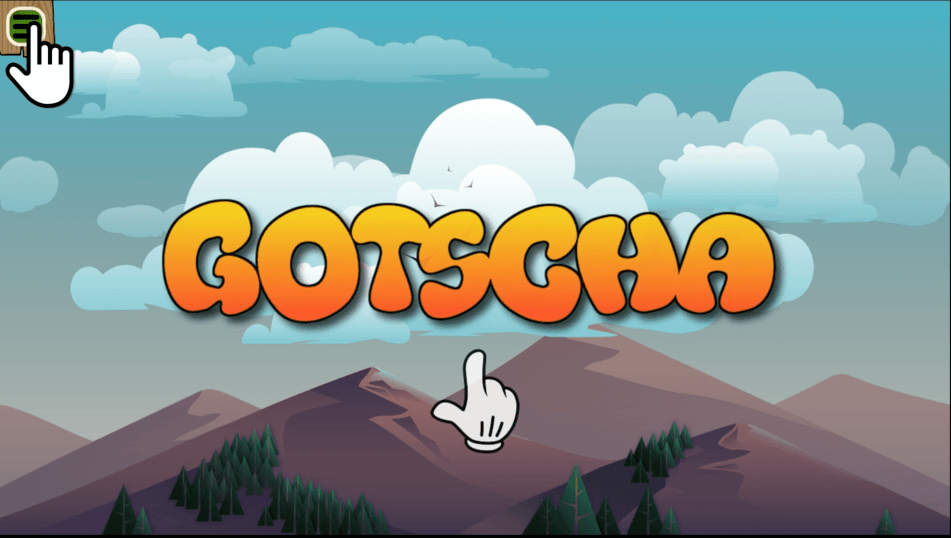
\includegraphics[width=1\textwidth]{figures/welcomescreen}
    \caption{Title Screen}
    \label{fig:titlescreen}
\end{figure}

\begin{figure}[H]
    \centering
    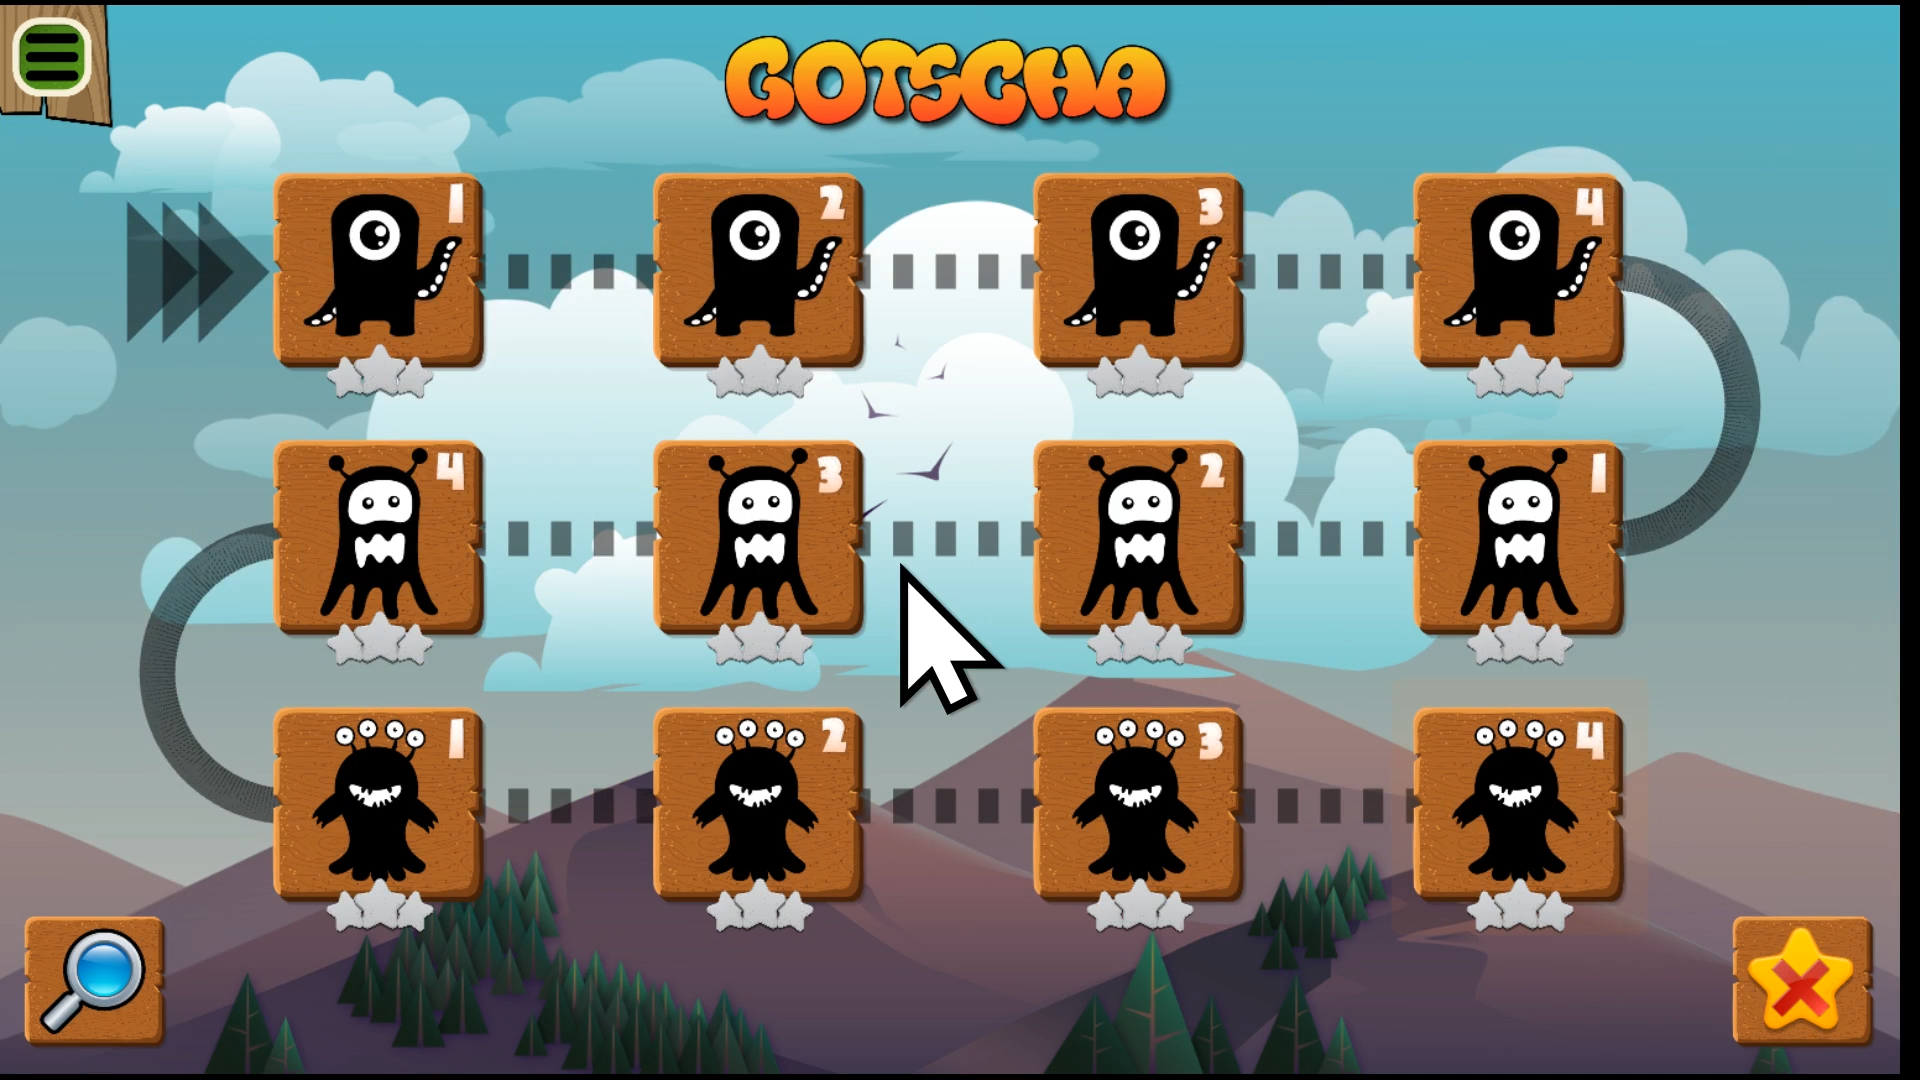
\includegraphics[width=1\textwidth]{figures/levelmenu}
    \caption{Level Menu}
    \label{fig:levelmenu}
\end{figure}

\begin{figure}[H]
    \centering
    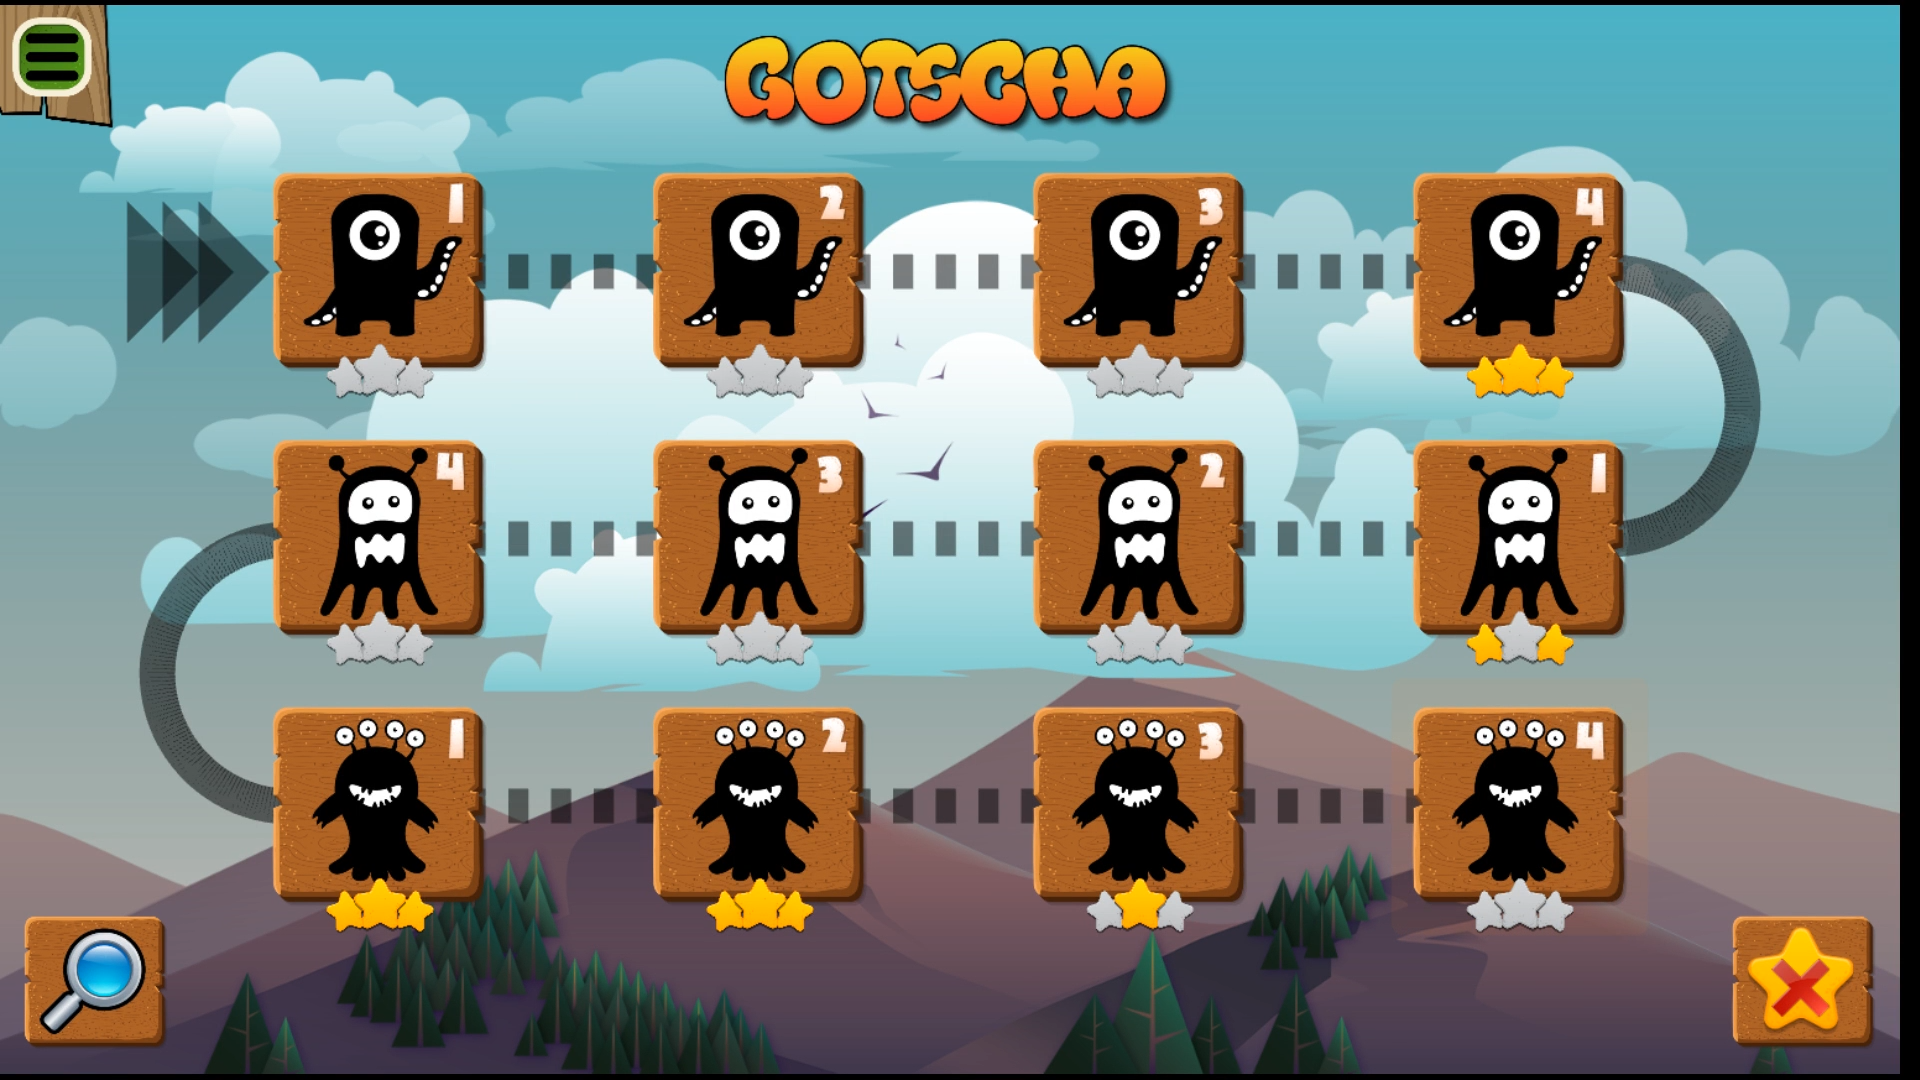
\includegraphics[width=1\textwidth]{figures/levelmenustars}
    \caption{Level Menu showing Stars}
    \label{fig:levelmenustars}
\end{figure}

\begin{figure}[H]
    \centering
    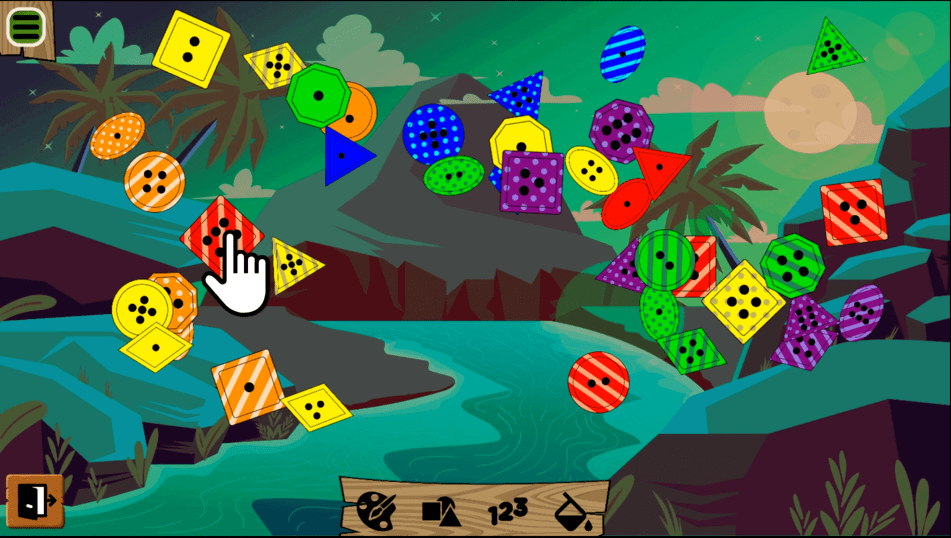
\includegraphics[width=1\textwidth]{figures/sortingscene1}
    \caption{Sorting Scene Category Mixture}
    \label{fig:sortingscene1}
\end{figure}

\begin{figure}[H]
    \centering
    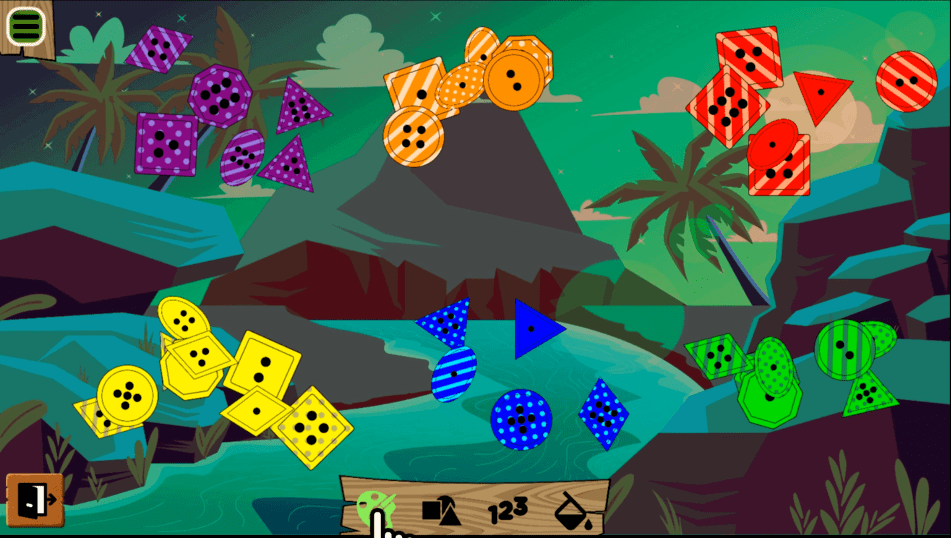
\includegraphics[width=1\textwidth]{figures/sortingscene2}
    \caption{Sorting Scene Category 1}
    \label{fig:sortingscene2}
\end{figure}

\begin{figure}[H]
    \centering
    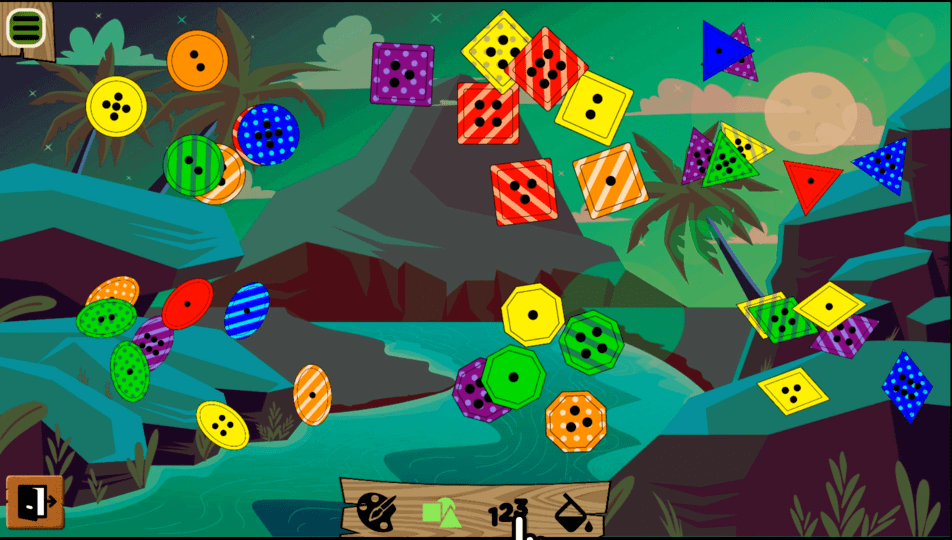
\includegraphics[width=1\textwidth]{figures/sortingscene3}
    \caption{Sorting Scene Category 2}
    \label{fig:sortingscene3}
\end{figure}

\begin{figure}[H]
    \centering
    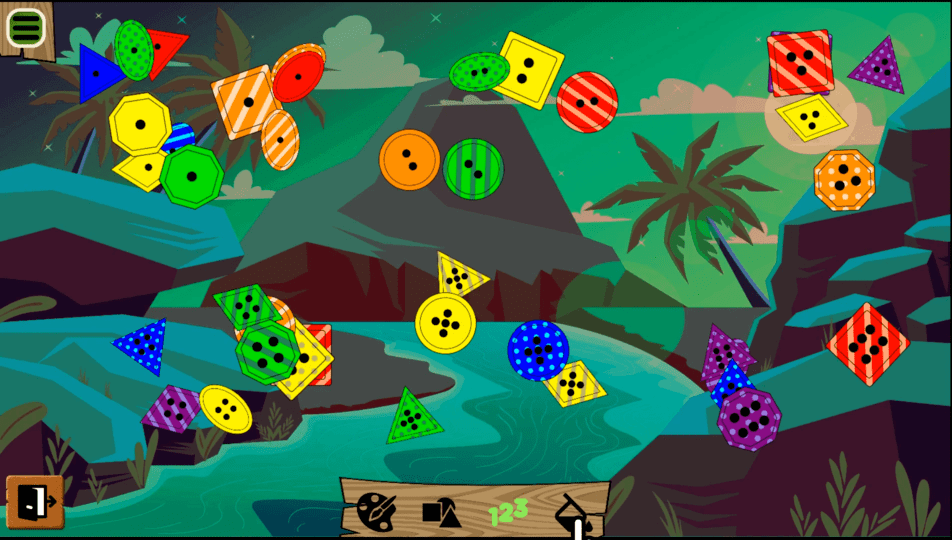
\includegraphics[width=1\textwidth]{figures/sortingscene4}
    \caption{Sorting Scene Category 3}
    \label{fig:sortingscene4}
\end{figure}

\begin{figure}[H]
    \centering
    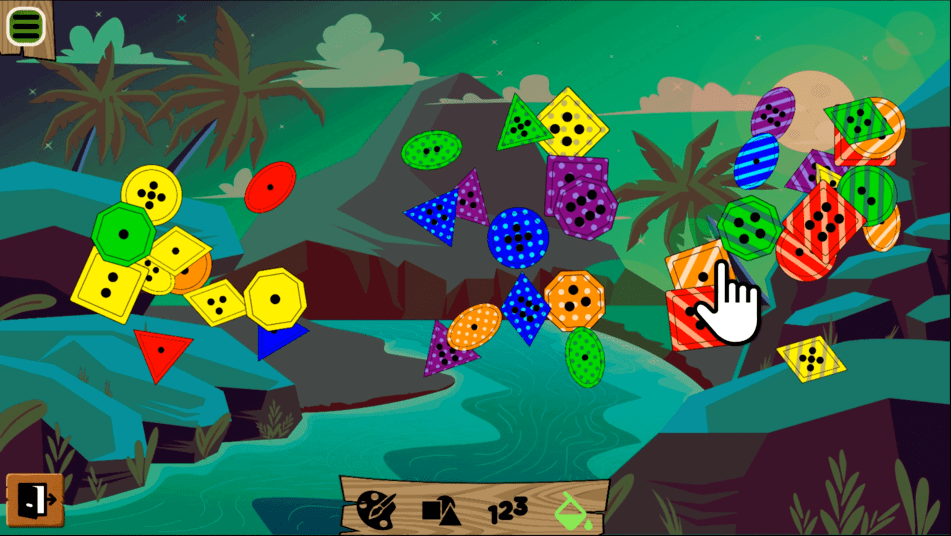
\includegraphics[width=1\textwidth]{figures/sortingscene5}
    \caption{Sorting Scene Category 4}
    \label{fig:sortingscene5}
\end{figure}

\begin{figure}[H]
    \centering
    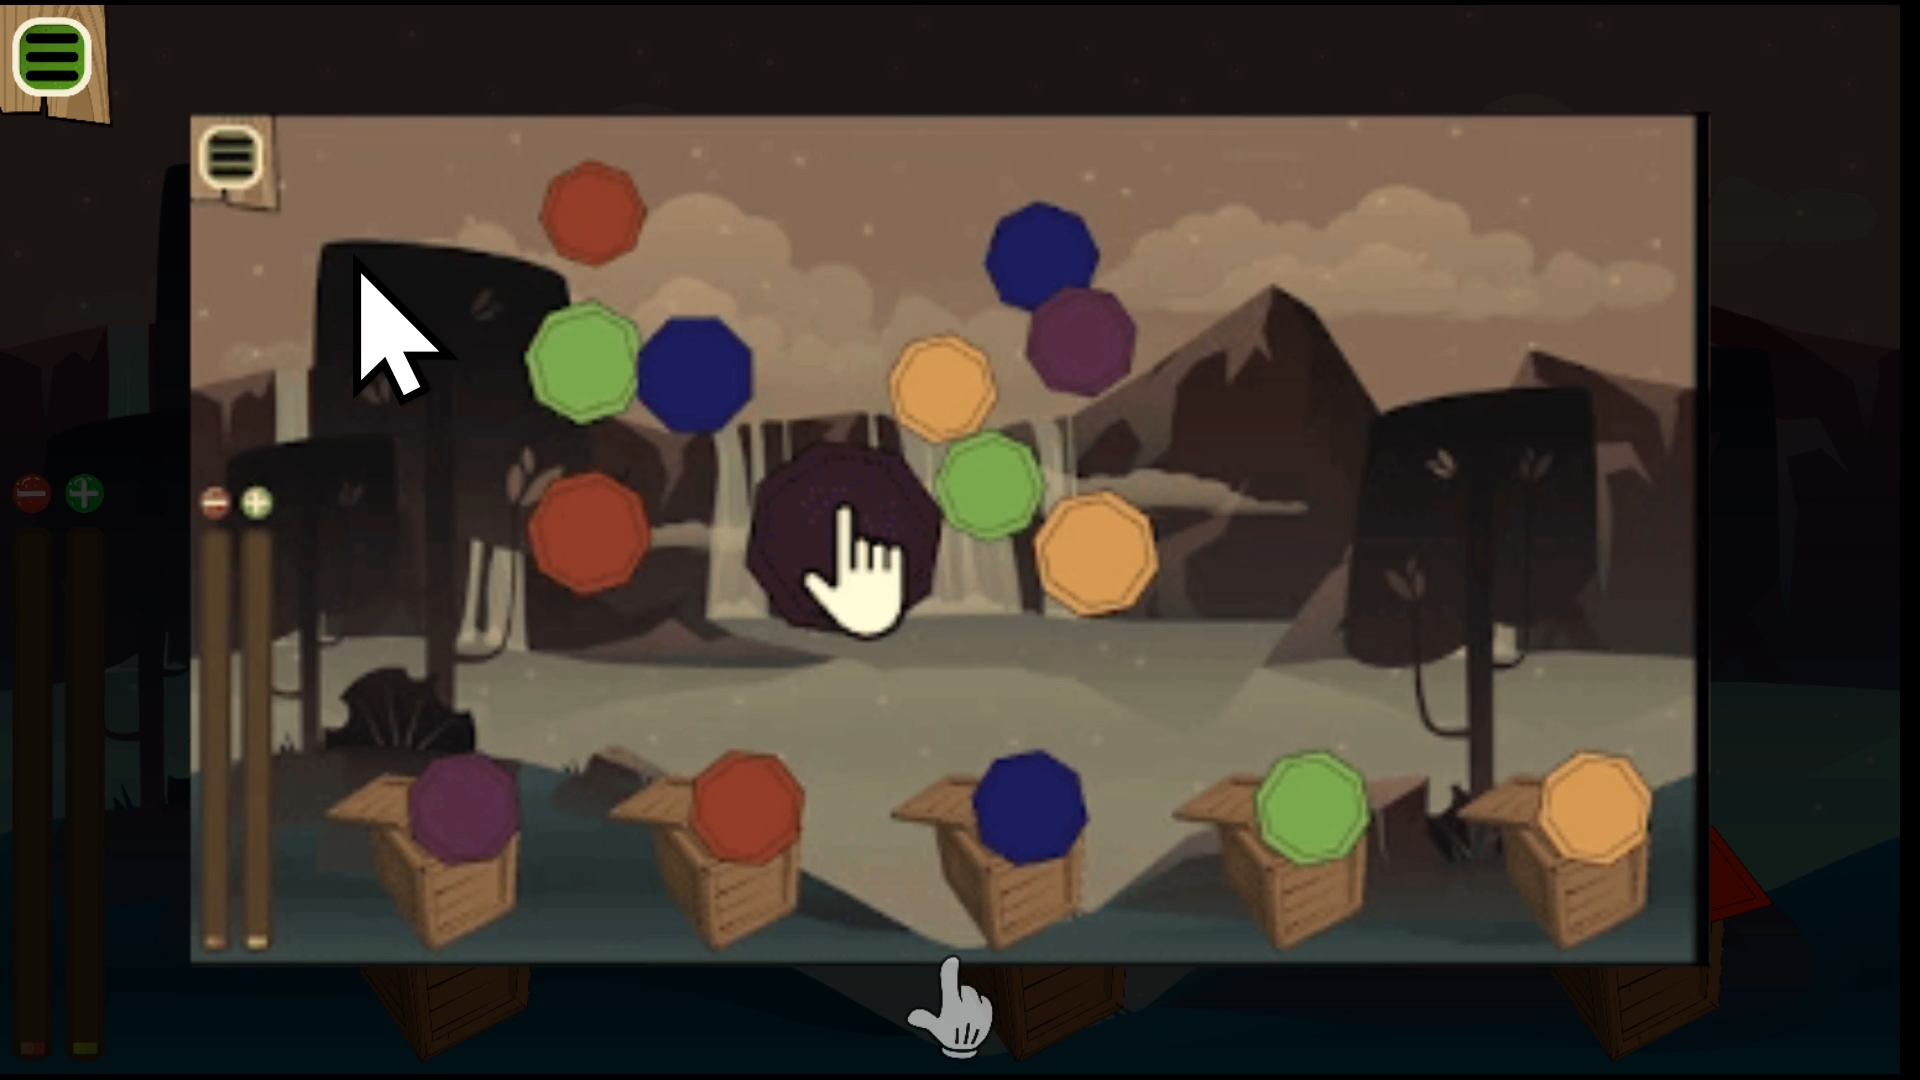
\includegraphics[width=1\textwidth]{figures/introduction}
    \caption{Introduction Screen to Sorting Scene}
    \label{fig:introduction}
\end{figure}

\begin{figure}[H]
    \centering
    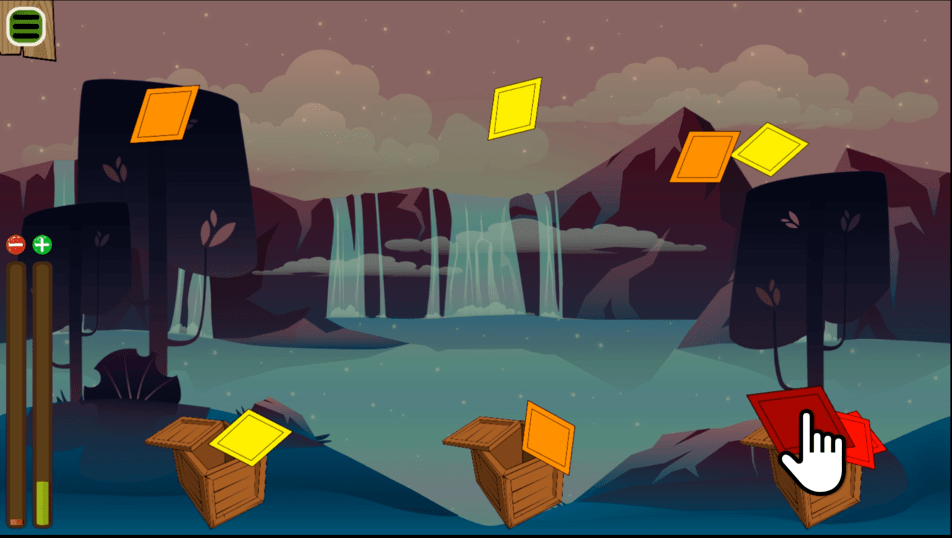
\includegraphics[width=1\textwidth]{figures/property1}
    \caption{Property Sorting Category 1}
    \label{fig:property1}
\end{figure}

\begin{figure}[H]
    \centering
    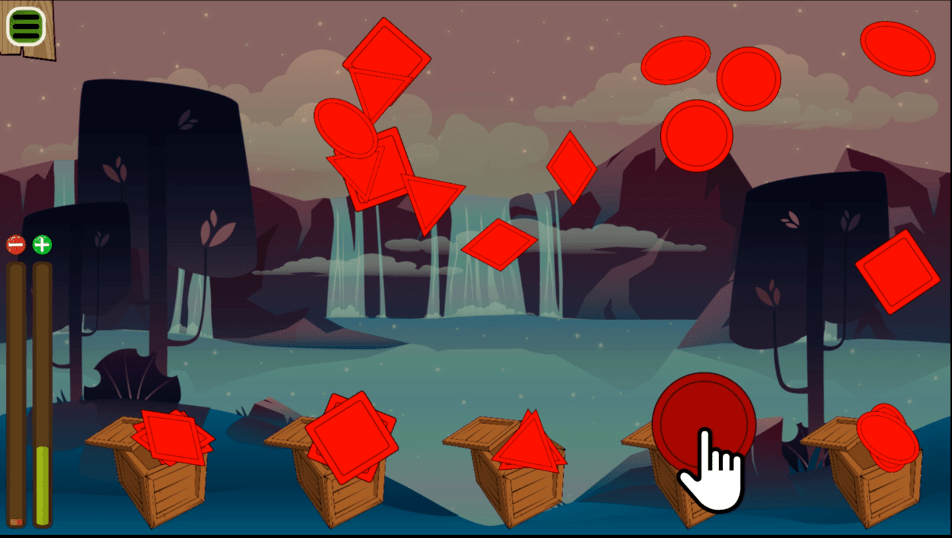
\includegraphics[width=1\textwidth]{figures/property2}
    \caption{Property Sorting Category 2}
    \label{fig:property2}
\end{figure}

\begin{figure}[H]
    \centering
    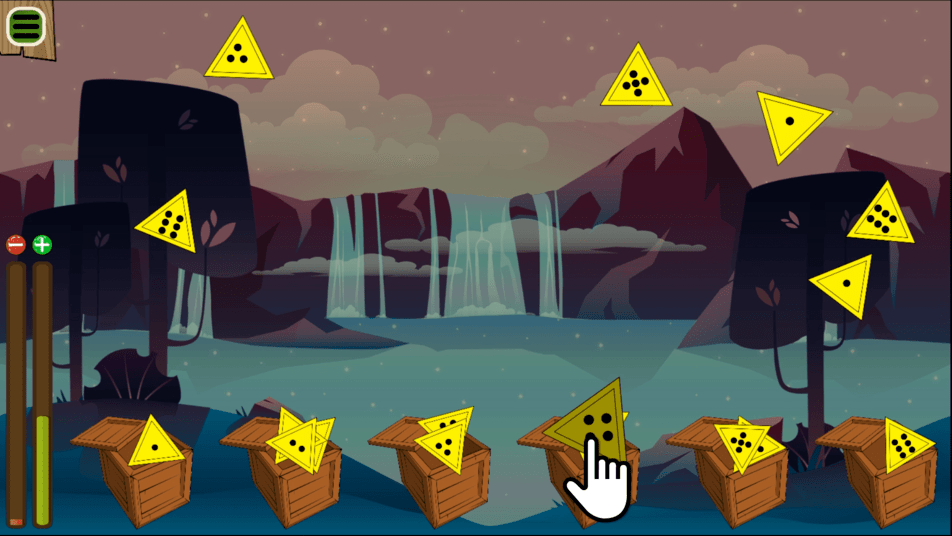
\includegraphics[width=1\textwidth]{figures/property3}
    \caption{Property Sorting Category 3}
    \label{fig:property3}
\end{figure}

\begin{figure}[H]
    \centering
    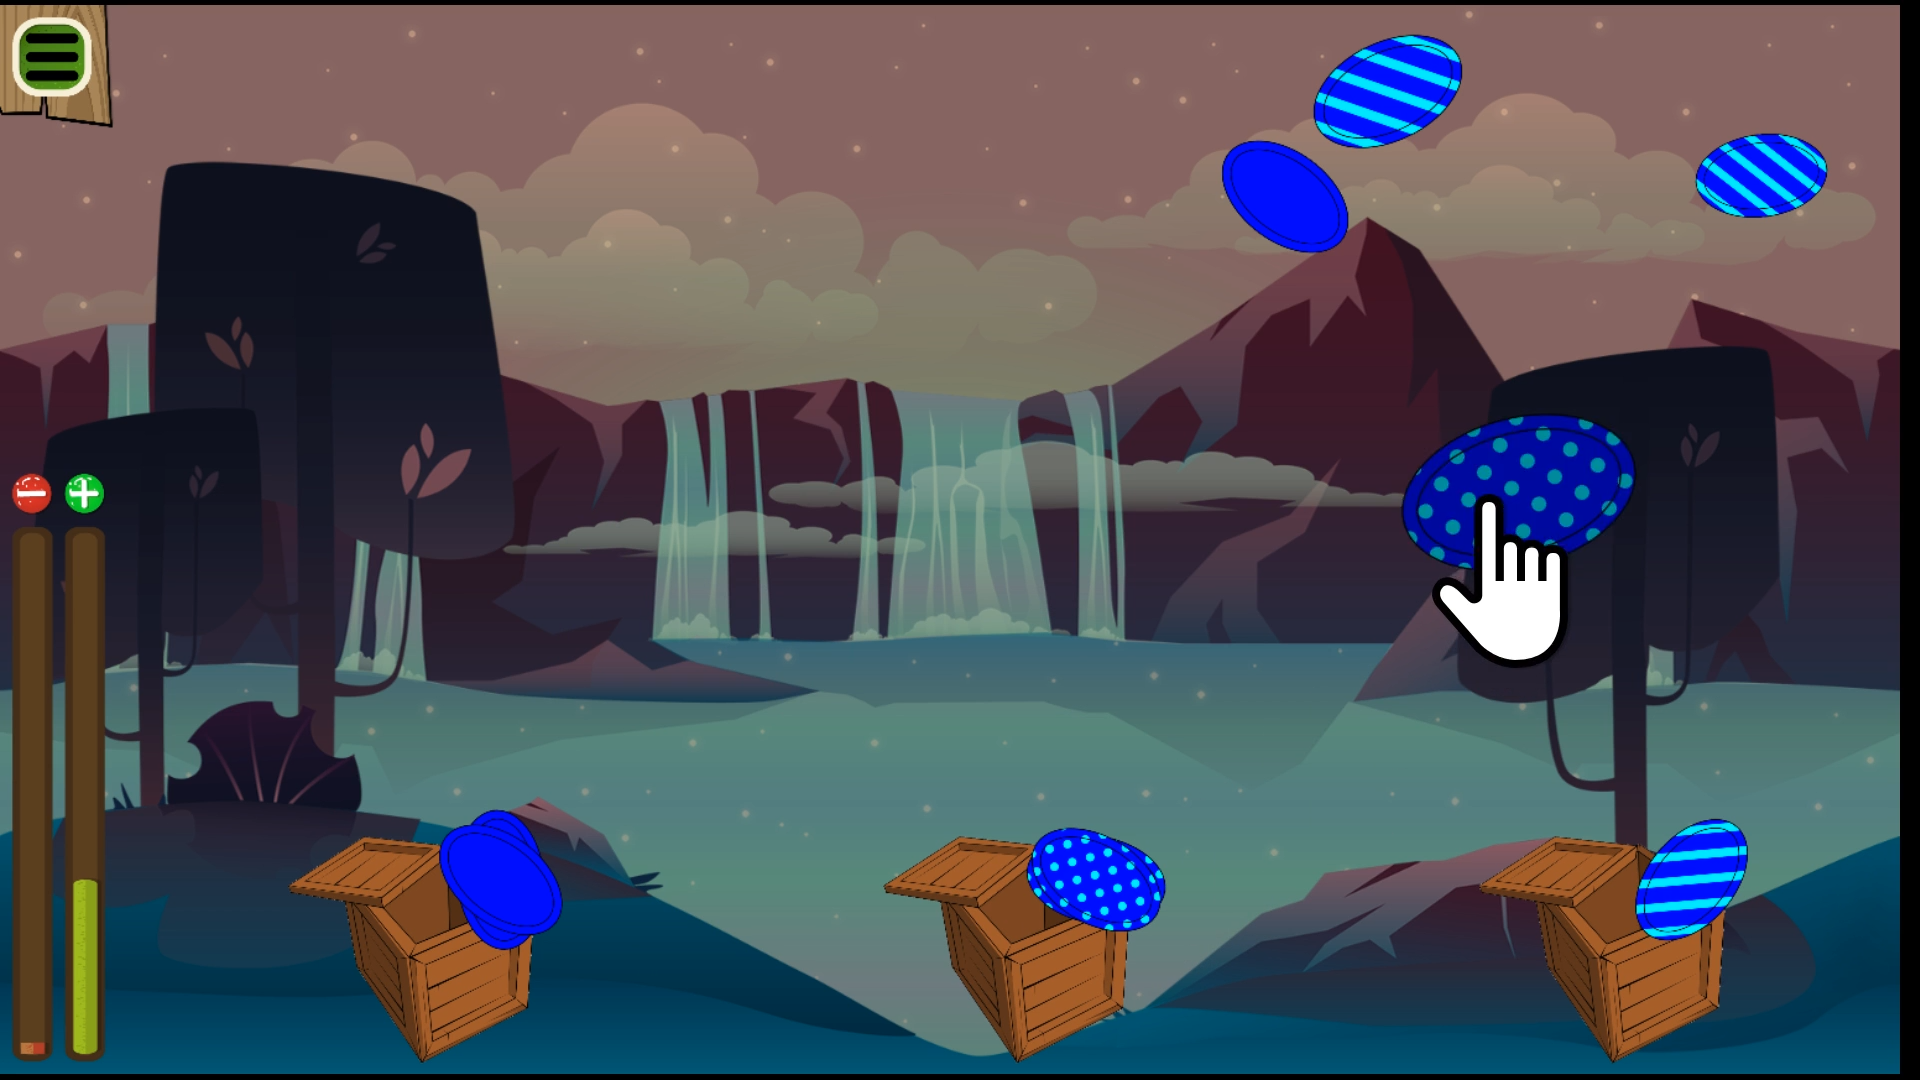
\includegraphics[width=1\textwidth]{figures/property4}
    \caption{Property Sorting Category 4}
    \label{fig:property4}
\end{figure}

\begin{figure}[H]
    \centering
    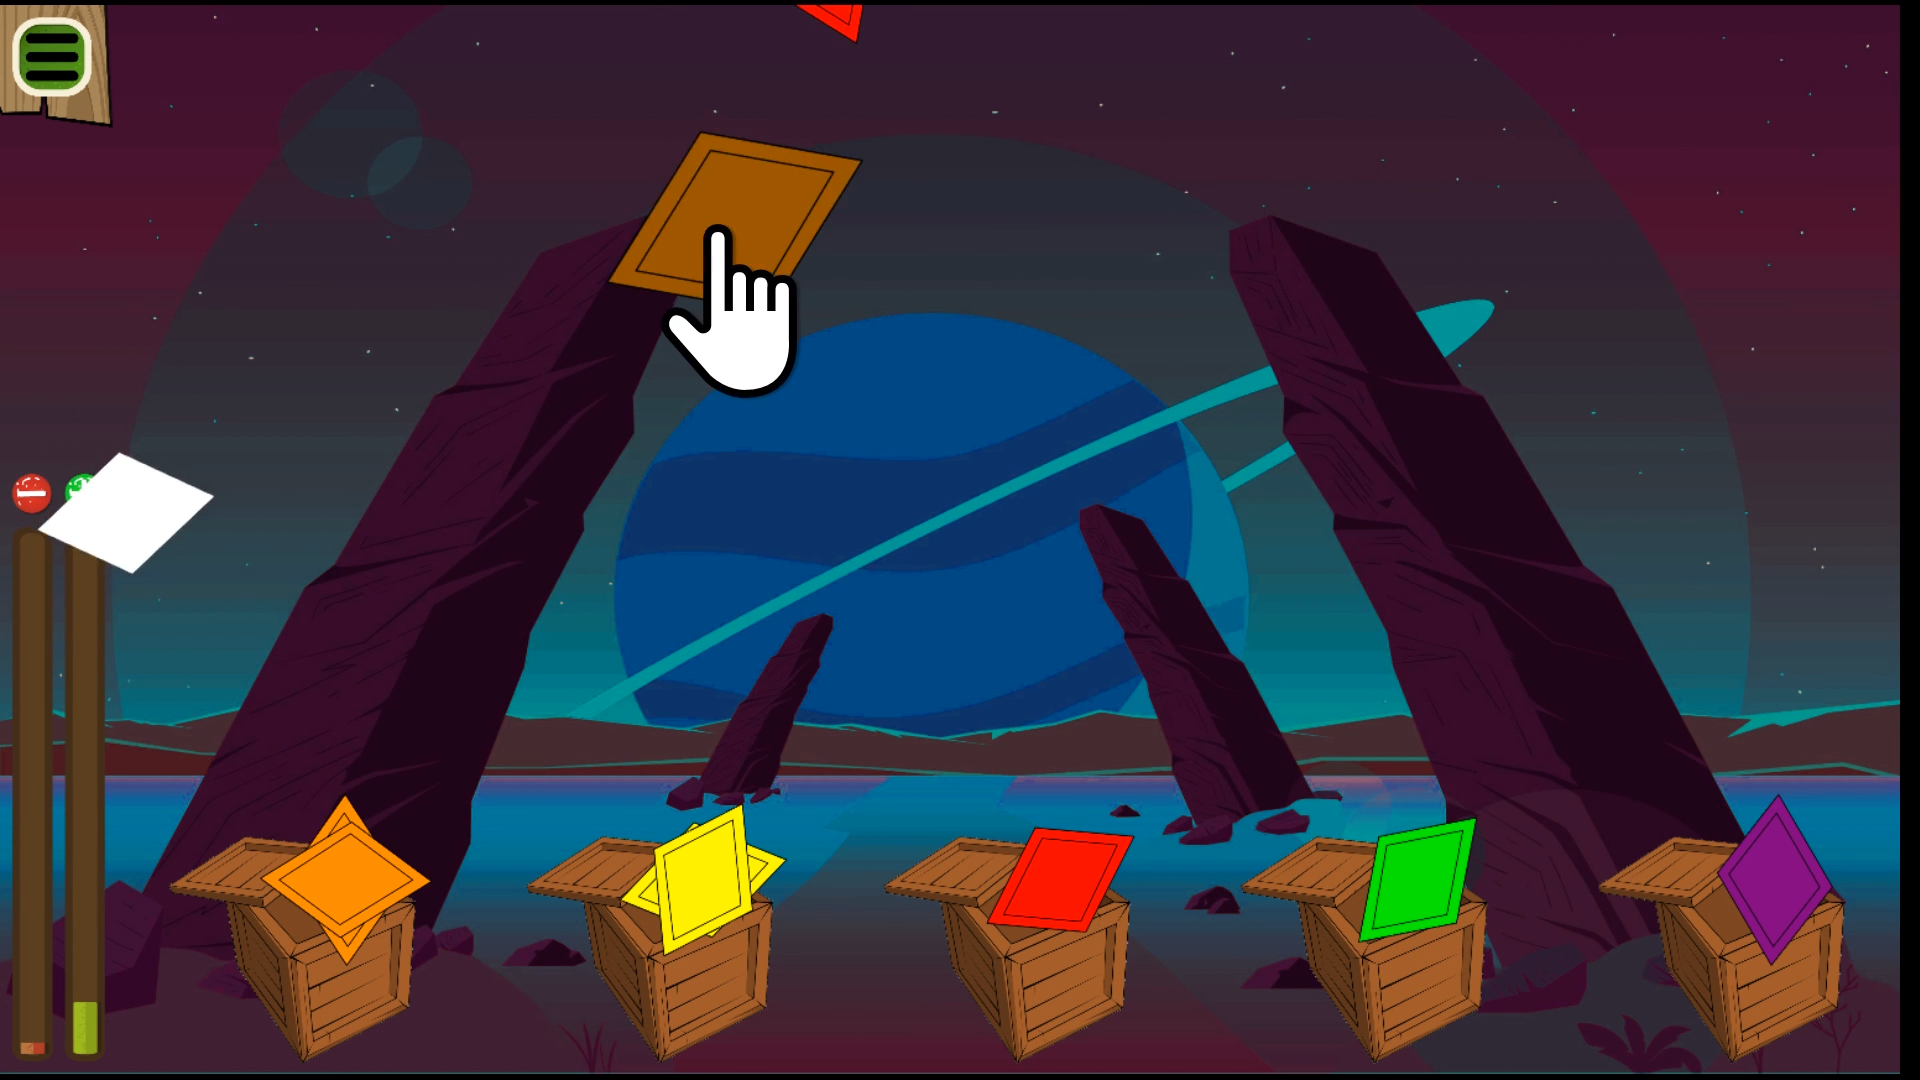
\includegraphics[width=1\textwidth]{figures/falling}
    \caption{Falling Property Sorting Category 1, 2--4 will be omitted}
    \label{fig:falling}
\end{figure}

\begin{figure}[H]
    \centering
    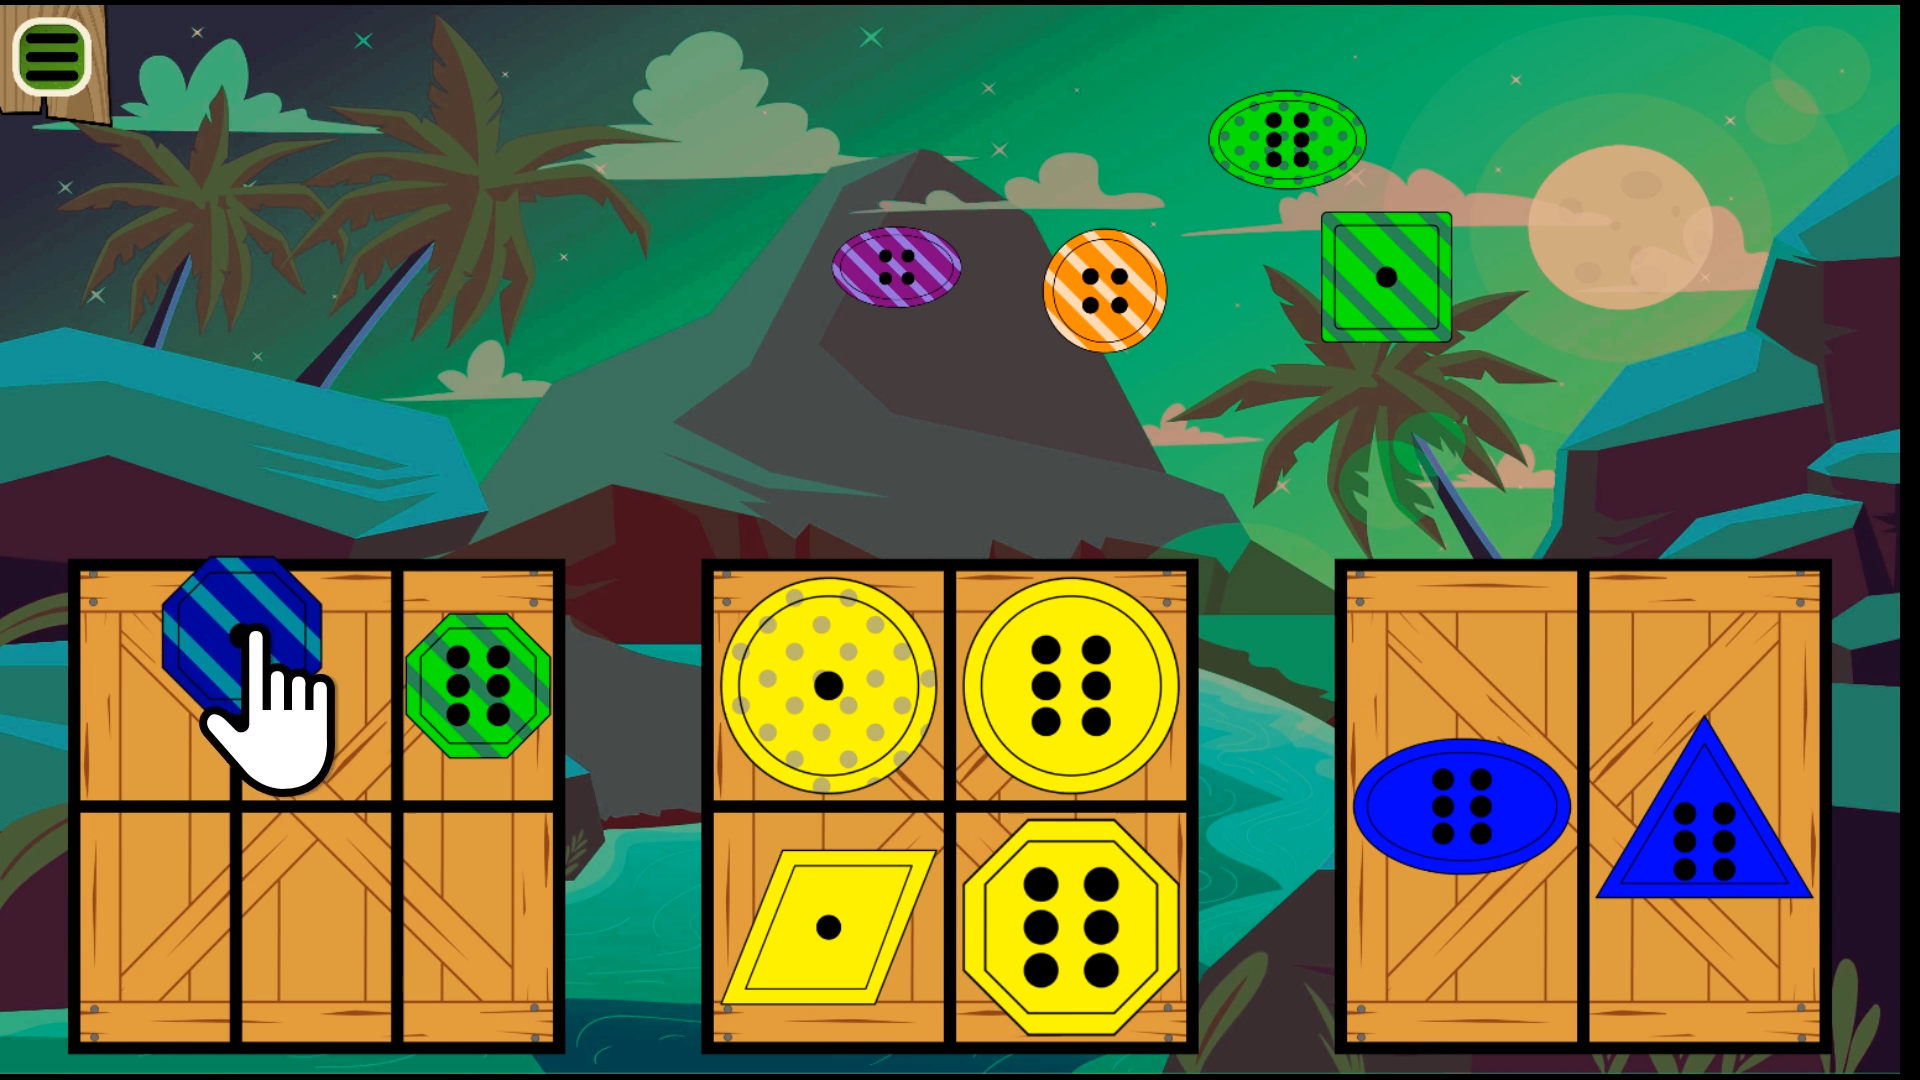
\includegraphics[width=1\textwidth]{figures/restricted1}
    \caption{Restricted Sorting Easy}
    \label{fig:restricted1}
\end{figure}

\begin{figure}[H]
    \centering
    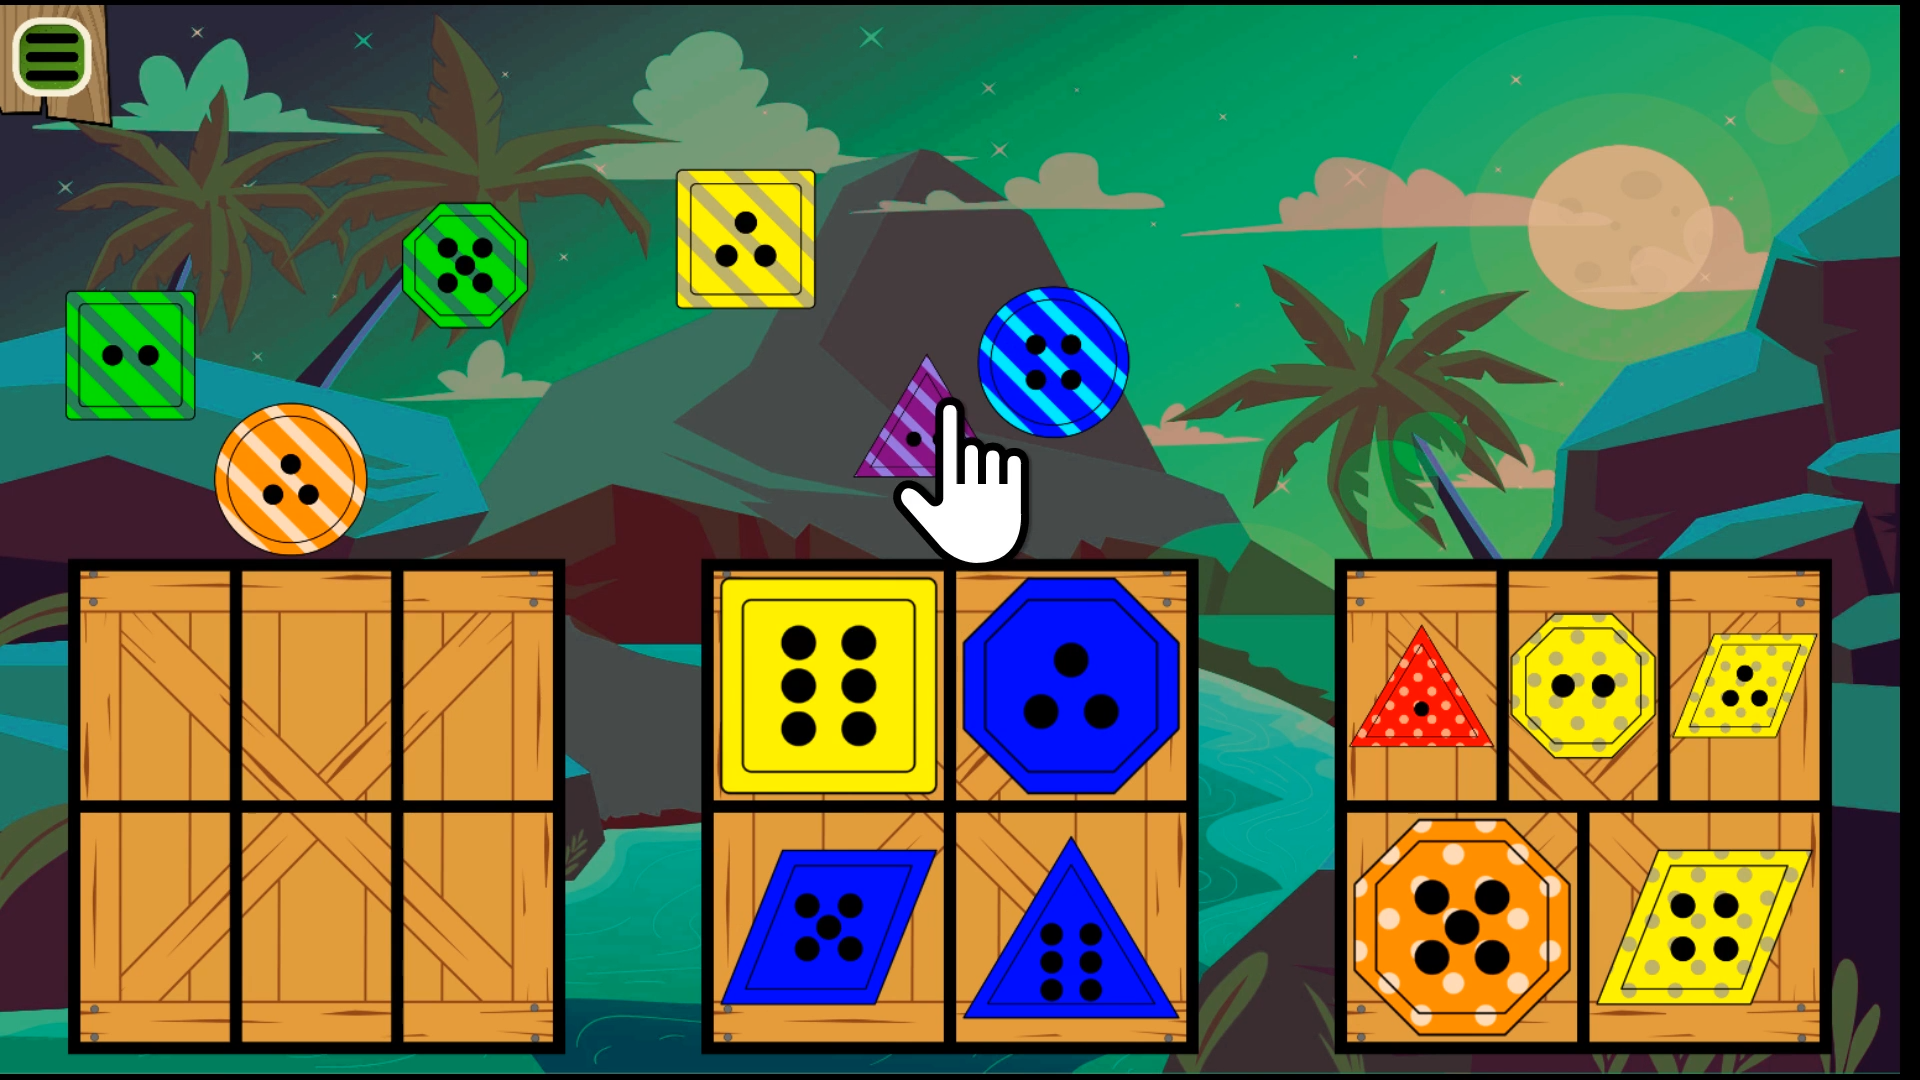
\includegraphics[width=1\textwidth]{figures/restricted2}
    \caption{Restricted Sorting 2 Hard}
    \label{fig:restricted2}
\end{figure}

\begin{figure}[H]
    \centering
    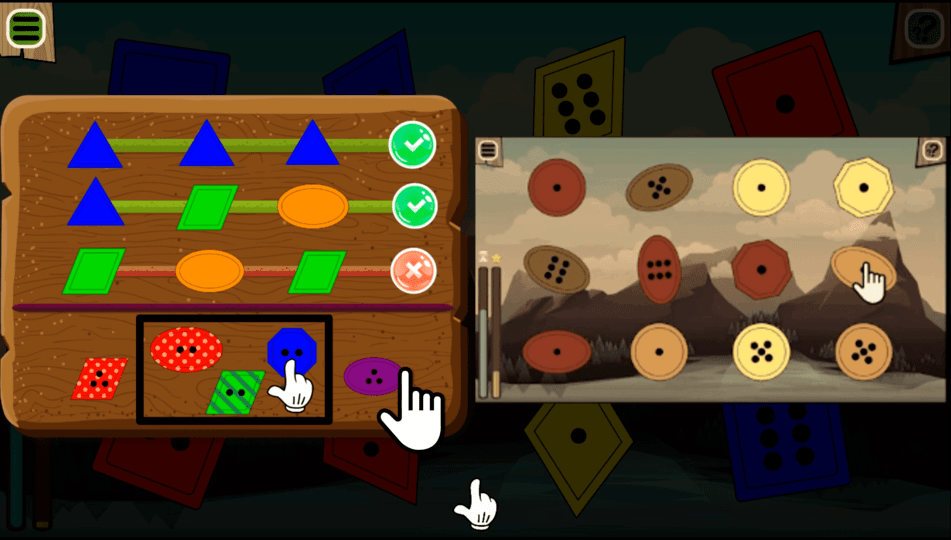
\includegraphics[width=1\textwidth]{figures/introgame}
    \caption{Introduction to Object Pairing Easy}
    \label{fig:introgame}
\end{figure}

\begin{figure}[H]
    \centering
    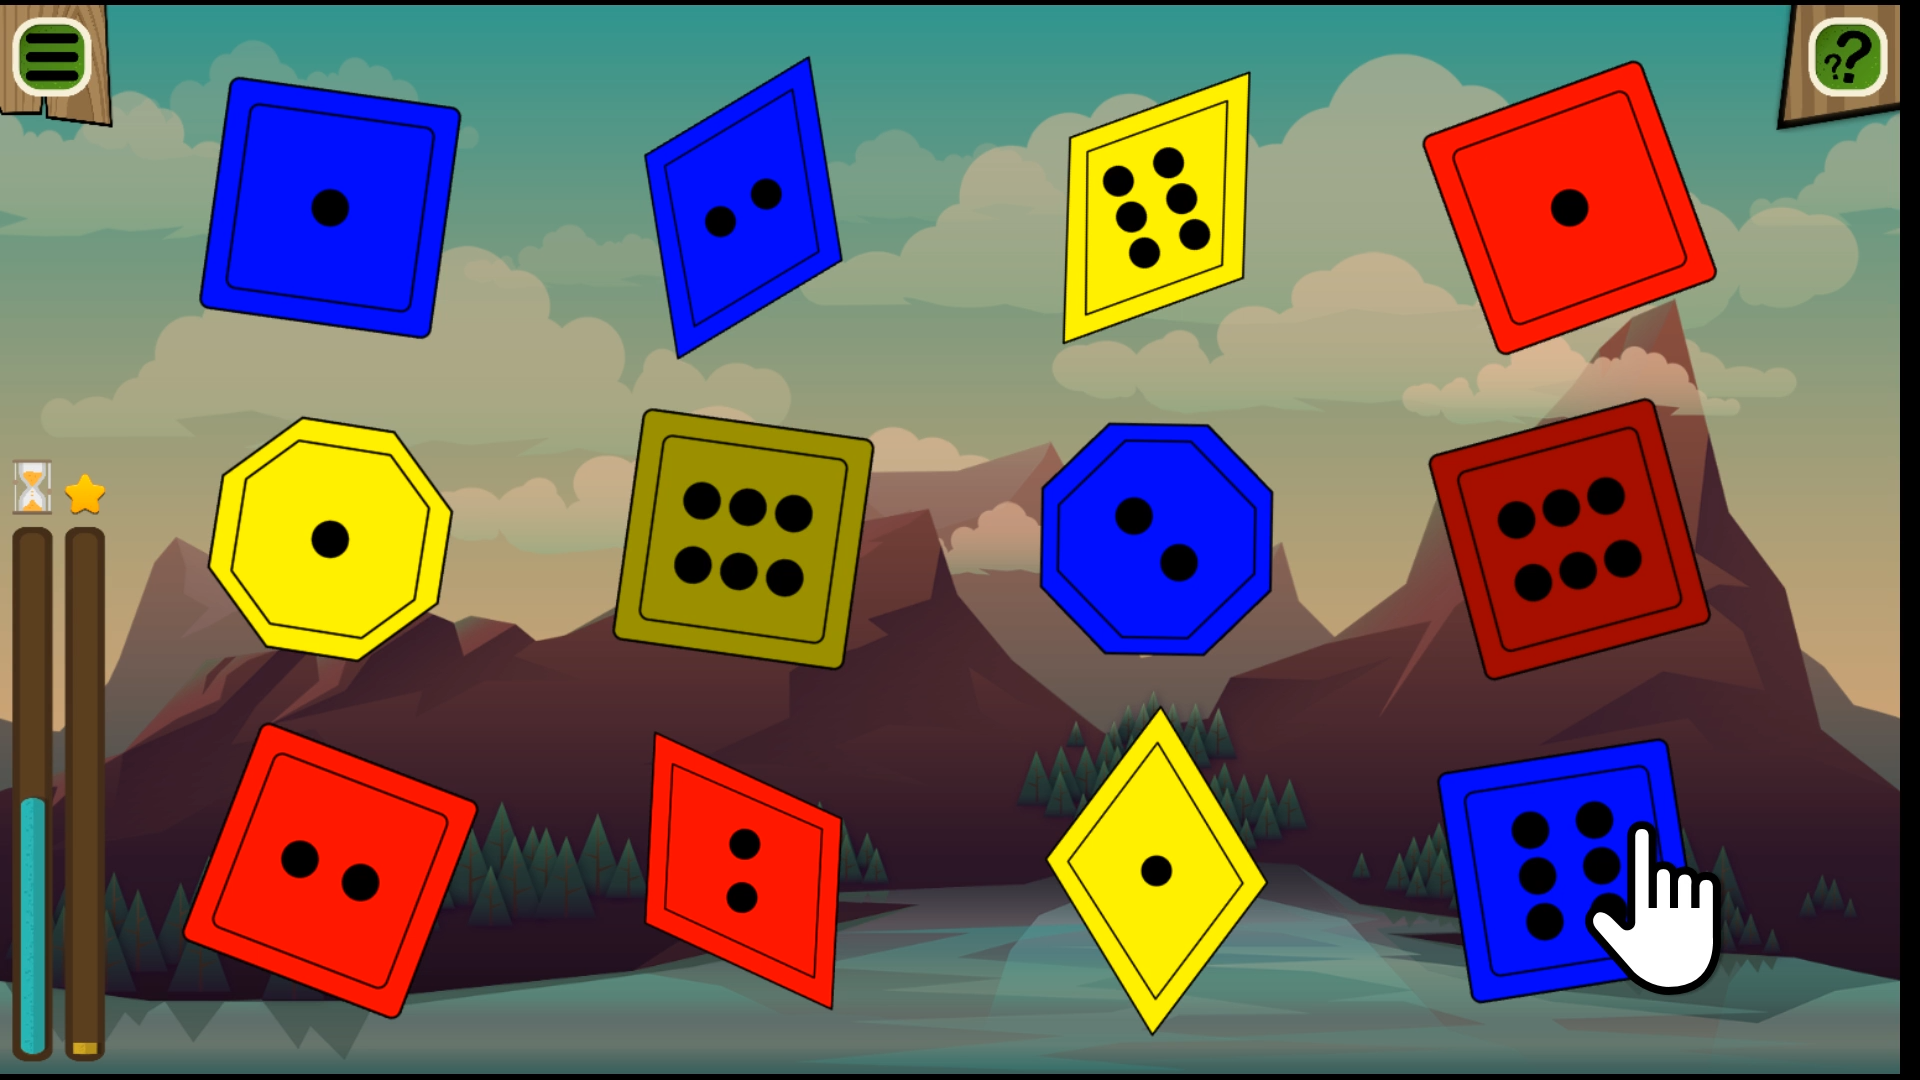
\includegraphics[width=1\textwidth]{figures/gameasy}
    \caption{Object Pairing Easy}
    \label{fig:gameeasy}
\end{figure}

\begin{figure}[H]
    \centering
    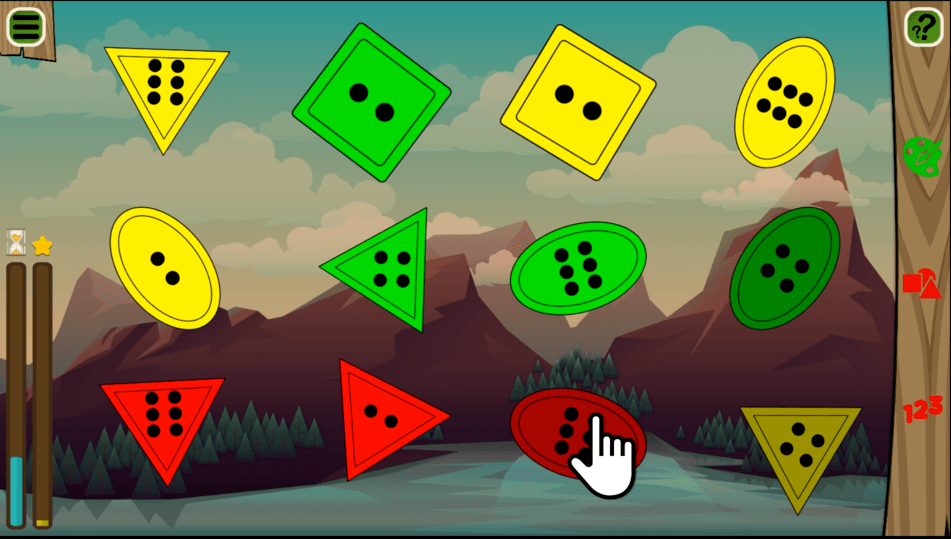
\includegraphics[width=1\textwidth]{figures/gameeasyhelp}
    \caption{Object Pairing Easy Helper Bar}
    \label{fig:gameeasyhelp}
\end{figure}

\begin{figure}[H]
    \centering
    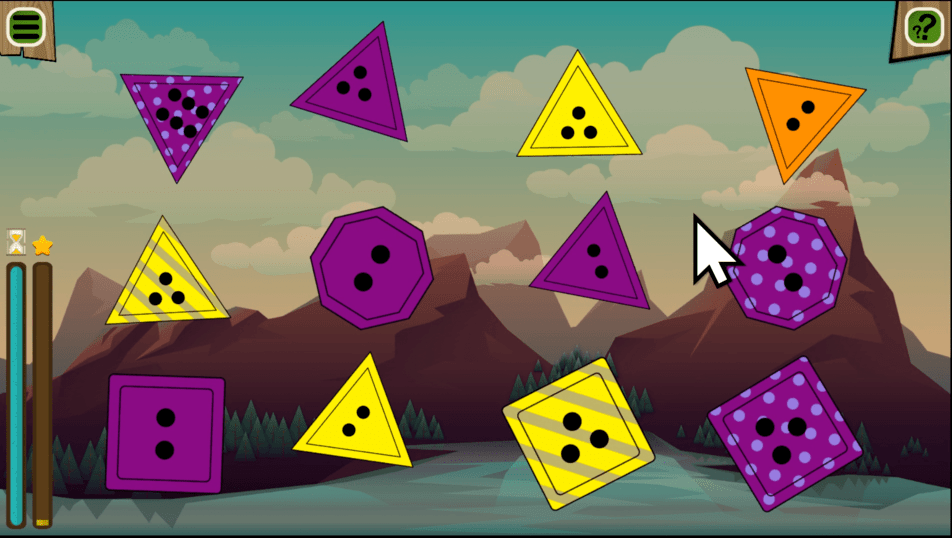
\includegraphics[width=1\textwidth]{figures/gamehard}
    \caption{Object Pairing Hard}
    \label{fig:gamehard}
\end{figure}

\begin{figure}[H]
    \centering
    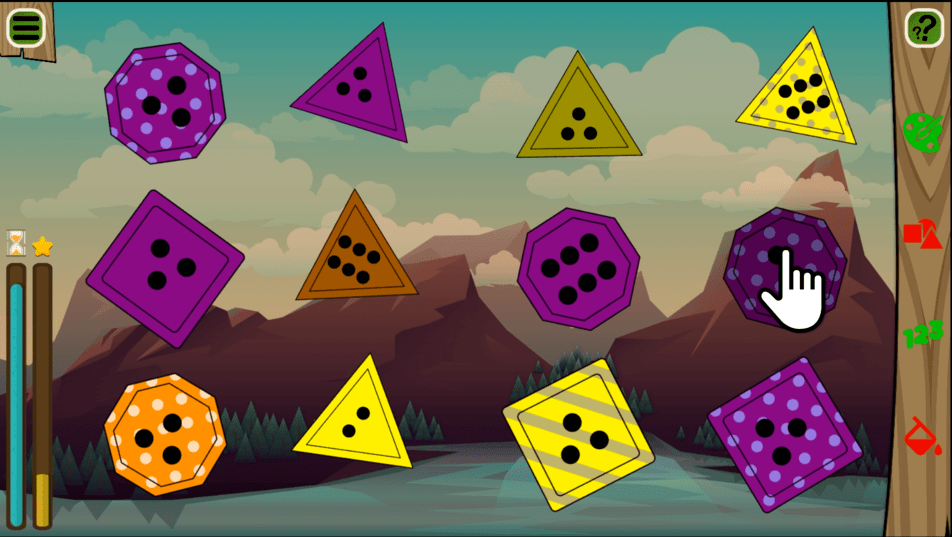
\includegraphics[width=1\textwidth]{figures/gamehardhelp}
    \caption{Object Pairing Hard Helper Bar}
    \label{fig:gamehardhelp}
\end{figure}

\begin{figure}[H]
    \centering
    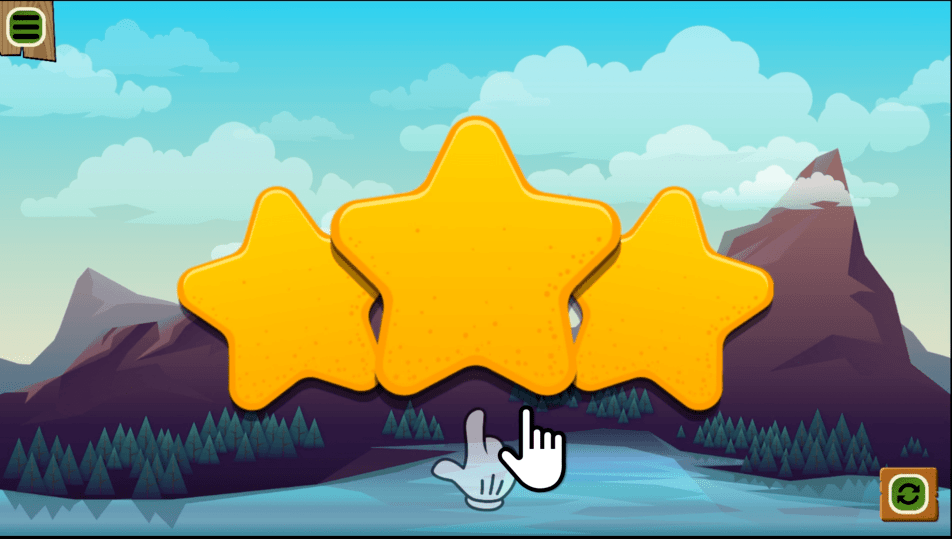
\includegraphics[width=1\textwidth]{figures/scorescreen}
    \caption{Score Screen}
    \label{fig:scorescreen}
\end{figure}
